
%% bare_conf.tex
%% V1.3
%% 2007/01/11
%% by Michael Shell
%% See:
%% http://www.michaelshell.org/
%% for current contact information.
%%
%% This is a skeleton file demonstrating the use of IEEEtran.cls
%% (requires IEEEtran.cls version 1.7 or later) with an IEEE conference paper.
%%
%% Support sites:
%% http://www.michaelshell.org/tex/ieeetran/
%% http://www.ctan.org/tex-archive/macros/latex/contrib/IEEEtran/
%% and
%% http://www.ieee.org/

%%*************************************************************************
%% Legal Notice:
%% This code is offered as-is without any warranty either expressed or
%% implied; without even the implied warranty of MERCHANTABILITY or
%% FITNESS FOR A PARTICULAR PURPOSE! 
%% User assumes all risk.
%% In no event shall IEEE or any contributor to this code be liable for
%% any damages or losses, including, but not limited to, incidental,
%% consequential, or any other damages, resulting from the use or misuse
%% of any information contained here.
%%
%% All comments are the opinions of their respective authors and are not
%% necessarily endorsed by the IEEE.
%%
%% This work is distributed under the LaTeX Project Public License (LPPL)
%% ( http://www.latex-project.org/ ) version 1.3, and may be freely used,
%% distributed and modified. A copy of the LPPL, version 1.3, is included
%% in the base LaTeX documentation of all distributions of LaTeX released
%% 2003/12/01 or later.
%% Retain all contribution notices and credits.
%% ** Modified files should be clearly indicated as such, including  **
%% ** renaming them and changing author support contact information. **
%%
%% File list of work: IEEEtran.cls, IEEEtran_HOWTO.pdf, bare_adv.tex,
%%                    bare_conf.tex, bare_jrnl.tex, bare_jrnl_compsoc.tex
%%*************************************************************************

% *** Authors should verify (and, if needed, correct) their LaTeX system  ***
% *** with the testflow diagnostic prior to trusting their LaTeX platform ***
% *** with production work. IEEE's font choices can trigger bugs that do  ***
% *** not appear when using other class files.                            ***
% The testflow support page is at:
% http://www.michaelshell.org/tex/testflow/



% Note that the a4paper option is mainly intended so that authors in
% countries using A4 can easily print to A4 and see how their papers will
% look in print - the typesetting of the document will not typically be
% affected with changes in paper size (but the bottom and side margins will).
% Use the testflow package mentioned above to verify correct handling of
% both paper sizes by the user's LaTeX system.
%
% Also note that the "draftcls" or "draftclsnofoot", not "draft", option
% should be used if it is desired that the figures are to be displayed in
% draft mode.
%
\documentclass[conference,11pt,single]{IEEEtran}
\usepackage{blindtext, graphicx}
\usepackage {cite}
\usepackage{setspace}
\graphicspath{ {diagrams/},{results/} }
\usepackage{subfigure}
% Add the compsoc option for Computer Society conferences.
%
% If IEEEtran.cls has not been installed into the LaTeX system files,
% manually specify the path to it like:
% \documentclass[conference]{../sty/IEEEtran}





% Some very useful LaTeX packages include:
% (uncomment the ones you want to load)


% *** MISC UTILITY PACKAGES ***
%
%\usepackage{ifpdf}
% Heiko Oberdiek's ifpdf.sty is very useful if you need conditional
% compilation based on whether the output is pdf or dvi.
% usage:
% \ifpdf
%   % pdf code
% \else
%   % dvi code
% \fi
% The latest version of ifpdf.sty can be obtained from:
% http://www.ctan.org/tex-archive/macros/latex/contrib/oberdiek/
% Also, note that IEEEtran.cls V1.7 and later provides a builtin
% \ifCLASSINFOpdf conditional that works the same way.
% When switching from latex to pdflatex and vice-versa, the compiler may
% have to be run twice to clear warning/error messages.






% *** CITATION PACKAGES ***
%
%\usepackage{cite}
% cite.sty was written by Donald Arseneau
% V1.6 and later of IEEEtran pre-defines the format of the cite.sty package
% \cite{} output to follow that of IEEE. Loading the cite package will
% result in citation numbers being automatically sorted and properly
% "compressed/ranged". e.g., [1], [9], [2], [7], [5], [6] without using
% cite.sty will become [1], [2], [5]--[7], [9] using cite.sty. cite.sty's
% \cite will automatically add leading space, if needed. Use cite.sty's
% noadjust option (cite.sty V3.8 and later) if you want to turn this off.
% cite.sty is already installed on most LaTeX systems. Be sure and use
% version 4.0 (2003-05-27) and later if using hyperref.sty. cite.sty does
% not currently provide for hyperlinked citations.
% The latest version can be obtained at:
% http://www.ctan.org/tex-archive/macros/latex/contrib/cite/
% The documentation is contained in the cite.sty file itself.






% *** GRAPHICS RELATED PACKAGES ***
%
\ifCLASSINFOpdf
  % \usepackage[pdftex]{graphicx}
  % declare the path(s) where your graphic files are
  % \graphicspath{{../pdf/}{../jpeg/}}
  % and their extensions so you won't have to specify these with
  % every instance of \includegraphics
  % \DeclareGraphicsExtensions{.pdf,.jpeg,.png}
\else
  % or other class option (dvipsone, dvipdf, if not using dvips). graphicx
  % will default to the driver specified in the system graphics.cfg if no
  % driver is specified.
  % \usepackage[dvips]{graphicx}
  % declare the path(s) where your graphic files are
  % \graphicspath{{../eps/}}
  % and their extensions so you won't have to specify these with
  % every instance of \includegraphics
  % \DeclareGraphicsExtensions{.eps}
\fi
% graphicx was written by David Carlisle and Sebastian Rahtz. It is
% required if you want graphics, photos, etc. graphicx.sty is already
% installed on most LaTeX systems. The latest version and documentation can
% be obtained at: 
% http://www.ctan.org/tex-archive/macros/latex/required/graphics/
% Another good source of documentation is "Using Imported Graphics in
% LaTeX2e" by Keith Reckdahl which can be found as epslatex.ps or
% epslatex.pdf at: http://www.ctan.org/tex-archive/info/
%
% latex, and pdflatex in dvi mode, support graphics in encapsulated
% postscript (.eps) format. pdflatex in pdf mode supports graphics
% in .pdf, .jpeg, .png and .mps (metapost) formats. Users should ensure
% that all non-photo figures use a vector format (.eps, .pdf, .mps) and
% not a bitmapped formats (.jpeg, .png). IEEE frowns on bitmapped formats
% which can result in "jaggedy"/blurry rendering of lines and letters as
% well as large increases in file sizes.
%
% You can find documentation about the pdfTeX application at:
% http://www.tug.org/applications/pdftex





% *** MATH PACKAGES ***
%
%\usepackage[cmex10]{amsmath}
% A popular package from the American Mathematical Society that provides
% many useful and powerful commands for dealing with mathematics. If using
% it, be sure to load this package with the cmex10 option to ensure that
% only type 1 fonts will utilized at all point sizes. Without this option,
% it is possible that some math symbols, particularly those within
% footnotes, will be rendered in bitmap form which will result in a
% document that can not be IEEE Xplore compliant!
%
% Also, note that the amsmath package sets \interdisplaylinepenalty to 10000
% thus preventing page breaks from occurring within multiline equations. Use:
%\interdisplaylinepenalty=2500
% after loading amsmath to restore such page breaks as IEEEtran.cls normally
% does. amsmath.sty is already installed on most LaTeX systems. The latest
% version and documentation can be obtained at:
% http://www.ctan.org/tex-archive/macros/latex/required/amslatex/math/





% *** SPECIALIZED LIST PACKAGES ***
%
\usepackage{algorithm}
\usepackage{algorithmic}
% algorithmic.sty was written by Peter Williams and Rogerio Brito.
% This package provides an algorithmic environment fo describing algorithms.
% You can use the algorithmic environment in-text or within a figure
% environment to provide for a floating algorithm. Do NOT use the algorithm
% floating environment provided by algorithm.sty (by the same authors) or
% algorithm2e.sty (by Christophe Fiorio) as IEEE does not use dedicated
% algorithm float types and packages that provide these will not provide
% correct IEEE style captions. The latest version and documentation of
% algorithmic.sty can be obtained at:
% http://www.ctan.org/tex-archive/macros/latex/contrib/algorithms/
% There is also a support site at:
% http://algorithms.berlios.de/index.html
% Also of interest may be the (relatively newer and more customizable)
% algorithmicx.sty package by Szasz Janos:
% http://www.ctan.org/tex-archive/macros/latex/contrib/algorithmicx/




% *** ALIGNMENT PACKAGES ***
%
%\usepackage{array}
% Frank Mittelbach's and David Carlisle's array.sty patches and improves
% the standard LaTeX2e array and tabular environments to provide better
% appearance and additional user controls. As the default LaTeX2e table
% generation code is lacking to the point of almost being broken with
% respect to the quality of the end results, all users are strongly
% advised to use an enhanced (at the very least that provided by array.sty)
% set of table tools. array.sty is already installed on most systems. The
% latest version and documentation can be obtained at:
% http://www.ctan.org/tex-archive/macros/latex/required/tools/


%\usepackage{mdwmath}
%\usepackage{mdwtab}
% Also highly recommended is Mark Wooding's extremely powerful MDW tools,
% especially mdwmath.sty and mdwtab.sty which are used to format equations
% and tables, respectively. The MDWtools set is already installed on most
% LaTeX systems. The lastest version and documentation is available at:
% http://www.ctan.org/tex-archive/macros/latex/contrib/mdwtools/


% IEEEtran contains the IEEEeqnarray family of commands that can be used to
% generate multiline equations as well as matrices, tables, etc., of high
% quality.


%\usepackage{eqparbox}
% Also of notable interest is Scott Pakin's eqparbox package for creating
% (automatically sized) equal width boxes - aka "natural width parboxes".
% Available at:
% http://www.ctan.org/tex-archive/macros/latex/contrib/eqparbox/





% *** SUBFIGURE PACKAGES ***
%\usepackage[tight,footnotesize]{subfigure}
% subfigure.sty was written by Steven Douglas Cochran. This package makes it
% easy to put subfigures in your figures. e.g., "Figure 1a and 1b". For IEEE
% work, it is a good idea to load it with the tight package option to reduce
% the amount of white space around the subfigures. subfigure.sty is already
% installed on most LaTeX systems. The latest version and documentation can
% be obtained at:
% http://www.ctan.org/tex-archive/obsolete/macros/latex/contrib/subfigure/
% subfigure.sty has been superceeded by subfig.sty.



%\usepackage[caption=false]{caption}
%\usepackage[font=footnotesize]{subfig}
% subfig.sty, also written by Steven Douglas Cochran, is the modern
% replacement for subfigure.sty. However, subfig.sty requires and
% automatically loads Axel Sommerfeldt's caption.sty which will override
% IEEEtran.cls handling of captions and this will result in nonIEEE style
% figure/table captions. To prevent this problem, be sure and preload
% caption.sty with its "caption=false" package option. This is will preserve
% IEEEtran.cls handing of captions. Version 1.3 (2005/06/28) and later 
% (recommended due to many improvements over 1.2) of subfig.sty supports
% the caption=false option directly:
%\usepackage[caption=false,font=footnotesize]{subfig}
%
% The latest version and documentation can be obtained at:
% http://www.ctan.org/tex-archive/macros/latex/contrib/subfig/
% The latest version and documentation of caption.sty can be obtained at:
% http://www.ctan.org/tex-archive/macros/latex/contrib/caption/




% *** FLOAT PACKAGES ***
%
%\usepackage{fixltx2e}
% fixltx2e, the successor to the earlier fix2col.sty, was written by
% Frank Mittelbach and David Carlisle. This package corrects a few problems
% in the LaTeX2e kernel, the most notable of which is that in current
% LaTeX2e releases, the ordering of single and double column floats is not
% guaranteed to be preserved. Thus, an unpatched LaTeX2e can allow a
% single column figure to be placed prior to an earlier double column
% figure. The latest version and documentation can be found at:
% http://www.ctan.org/tex-archive/macros/latex/base/



%\usepackage{stfloats}
% stfloats.sty was written by Sigitas Tolusis. This package gives LaTeX2e
% the ability to do double column floats at the bottom of the page as well
% as the top. (e.g., "\begin{figure*}[!b]" is not normally possible in
% LaTeX2e). It also provides a command:
%\fnbelowfloat
% to enable the placement of footnotes below bottom floats (the standard
% LaTeX2e kernel puts them above bottom floats). This is an invasive package
% which rewrites many portions of the LaTeX2e float routines. It may not work
% with other packages that modify the LaTeX2e float routines. The latest
% version and documentation can be obtained at:
% http://www.ctan.org/tex-archive/macros/latex/contrib/sttools/
% Documentation is contained in the stfloats.sty comments as well as in the
% presfull.pdf file. Do not use the stfloats baselinefloat ability as IEEE
% does not allow \baselineskip to stretch. Authors submitting work to the
% IEEE should note that IEEE rarely uses double column equations and
% that authors should try to avoid such use. Do not be tempted to use the
% cuted.sty or midfloat.sty packages (also by Sigitas Tolusis) as IEEE does
% not format its papers in such ways.





% *** PDF, URL AND HYPERLINK PACKAGES ***
%
%\usepackage{url}
% url.sty was written by Donald Arseneau. It provides better support for
% handling and breaking URLs. url.sty is already installed on most LaTeX
% systems. The latest version can be obtained at:
% http://www.ctan.org/tex-archive/macros/latex/contrib/misc/
% Read the url.sty source comments for usage information. Basically,
% \url{my_url_here}.





% *** Do not adjust lengths that control margins, column widths, etc. ***
% *** Do not use packages that alter fonts (such as pslatex).         ***
% There should be no need to do such things with IEEEtran.cls V1.6 and later.
% (Unless specifically asked to do so by the journal or conference you plan
% to submit to, of course. )


% correct bad hyphenation here
\hyphenation{op-tical net-works semi-conduc-tor}

\singlespacing
\IEEEoverridecommandlockouts
\begin{document}

%
% paper title
% can use linebreaks \\ within to get better formatting as desired
\title{
    Towards Clustering Graph Representation of Geographic Dataset for Distributed Systems\\
}

\author{
    \begin{tabular}{ccc}
    Subhadeep Bhattacharya$^\dag$ & Fahim Chowdhury$^\dag$ & Rupak Roy$^\dag$\\
    \end{tabular}  \\
%    \hspace{1pc}~\\
    \begin{tabular}{c}
    Florida State University$^\dag$ \\
    {\{bhattach,fchowdhu,rroy\}@cs.fsu.edu} \\
    \end{tabular}
}

%\and
%\IEEEauthorblockN{Weikuan Yu}
%\IEEEauthorblockA{Department of Computer Science\\
%Florida State University\\
%\textit{yuw@cs.fsu.edu}}}

% conference papers do not typically use \thanks and this command
% is locked out in conference mode. If really needed, such as for
% the acknowledgment of grants, issue a \IEEEoverridecommandlockouts
% after \documentclass

% for over three affiliations, or if they all won't fit within the width
% of the page, use this alternative format:
% 
%\author{\IEEEauthorblockN{Michael Shell\IEEEauthorrefmark{1},
%Homer Simpson\IEEEauthorrefmark{2},
%James Kirk\IEEEauthorrefmark{3}, 
%Montgomery Scott\IEEEauthorrefmark{3} and
%Eldon Tyrell\IEEEauthorrefmark{4}}
%\IEEEauthorblockA{\IEEEauthorrefmark{1}School of Electrical and Computer Engineering\\
%Georgia Institute of Technology,
%Atlanta, Georgia 30332--0250\\ Email: see http://www.michaelshell.org/contact.html}
%\IEEEauthorblockA{\IEEEauthorrefmark{2}Twentieth Century Fox, Springfield, USA\\
%Email: homer@thesimpsons.com}
%\IEEEauthorblockA{\IEEEauthorrefmark{3}Starfleet Academy, San Francisco, California 96678-2391\\
%Telephone: (800) 555--1212, Fax: (888) 555--1212}
%\IEEEauthorblockA{\IEEEauthorrefmark{4}Tyrell Inc., 123 Replicant Street, Los Angeles, California 90210--4321}}

% use for special paper notices
%\IEEEspecialpapernotice{(Invited Paper)}

% make the title area
\maketitle



% IEEEtran.cls defaults to using nonbold math in the Abstract.
% This preserves the distinction between vectors and scalars. However,
% if the journal you are submitting to favors bold math in the abstract,
% then you can use LaTeX's standard command \boldmath at the very start
% of the abstract to achieve this. Many IEEE journals frown on math
% in the abstract anyway.

% Note that keywords are not normally used for peerreview papers.
%\begin{IEEEkeywords}
%IEEEtran, journal, \LaTeX, paper, template.
%\end{IEEEkeywords}






% For peer review papers, you can put extra information on the cover
% page as needed:
% \ifCLASSOPTIONpeerreview
% \begin{center} \bfseries EDICS Category: 3-BBND \end{center}
% \fi
%
% For peerreview papers, this IEEEtran command inserts a page break and
% creates the second title. It will be ignored for other modes.
\IEEEpeerreviewmaketitle

Please note\footnote{The authors are listed in alphabetic order of the last name. All the authors have equal contribution.}
\section{Introduction}
\label{sec:introduction}

Graph representation of huge dataset used for solving real world problems
is a popular format to feed computable data to the datamining applications.
Oftentimes, these data structures can be complicated with respect to its
connectivity among the elements of the representation. This dependency
among the datapoints or nodes of the graph not only makes it a complex task
to extract the insights from the data through datamining, but also renders
the application workflow as a hindrance to the parallelization for
efficiently leveraging high performance computing (HPC) infrastructures.
The goal of the project is to perform research on applying clustering
techniques on large graph representation of huge real world dataset
in order to maximize data parallelism in the datamining models for
utilizing HPC resources while ensuring reasonable accuracy of the system.

In particular, the research intends to initialize satisfying the general
motivation of applying graph clustering to improve parallelism
by focusing into a special and narrow sector as a proof of concept.
This sector deals with feeding large geographic map data to a system
for preprocessing and formatting the data in graph representation
where a coordinate, i.e., tuple of longitude and lattitude of
a specific geographic point, is treated as a node and the connecting
road between two coordinates is presented as the edge.
This large graph presenting the map can be used by the system to
solve different problems in the transportation system. For example,
this data can be used for finding the shortest path between two points of the graph.

Using legacy algorithms like Dijkstra's algorithm or even comparatively
more modern techniques like A* search will pose
immense time complexity if run on sequential systems.
Performance maximization via using distributed HPC systems can only be possible
if divide and conquer strategy can be applied on the data representation
by clustering the graph into smaller chunks and run the algorithm
upon the lower volume data in parallel, and finally combining
all the small results to deduce the final outcome.

Taking all these research requirements into consideration, this project proposes the following contributions.
\begin{itemize}
	\item A thorough survey on the state-of-the-art graph clustering techniques in general.
	\item Application of different graph clustering on huge geographic data as a special case handling.
	\item Execution of a shortest path algorithm as a proof of concept for evaluating the efficacy of different clustering techniques.
	\item Verification of performance and accuracy of the application for different clustering on HPC systems via thorough experiments.
	\item Comparison among different clustering techniques and recommendation for the specific data workload in concern, i.e. geographic map data.
\end{itemize}

\section{Literature Survey}
\label{sec:literature_survey}

Clustering the graph representation for geographical dataset continues to gain 
huge attention as it shows its potential for solving many real world problems. 
However, time taken by the graph algorithms is still an important challenge for 
real-time analysis which can be minimized by using the HPC infrastructure.
In~\cite{parallel_graph_algorithm} Bogle et. al. presents a new 
distributed-memory, BFS based parallel algorithm to identify and remove 
disconnected components or hinge vertices for graph-algorithms while 
significantly improving the convergence of iterative solvers. This work is 
extremely related in our context as the objective is to develop an efficient 
and accurate parallel algorithm for geographical dataset using its graphical 
representation.

Clustering the graphs in each node plays an important role in solving this 
scenario and state of the art researches 
need to be explored in this regard. Efficient semi-supervised learning can be 
one of the choice while doing the graph 
clustering.
Dhillon et. al.~\cite{kernel_kmeans} shows semi-supervised learning can improve 
the  graph 
clustering results and states an objective function for weighted kernel k-means 
by using Hidden Markov Random Fields, certain class of constraint penalty 
function and squared Euclidean Distance. 
Kulis et. al.~\cite{semi_supervised_graph_clustering} proposes SS-KERNELKMEANS 
to optimize a semi-supervised clustering objective for graph-base inputs by 
proposing a more generalized formulation and also exhibits an equivalence 
between the kernel k-means objective function
and a special case of the HMRF-based
semi-supervised clustering objective.

Detecting densely connected groups in a large graph is also a primary 
requirement in our approach. Zhou et. 
al.~\cite{structural_attribute_similarity_clustering} proposes SA-Cluster, a 
novel graph clustering algorithm based on both structural and attribute 
similarities using a unified distance measure. This method considers the 
heterogeneous vertex properties apart from the overall topological structure 
for clustering and shows its effectiveness both theoritically and 
experimentally.

Even the possibilities of using deep learning in graph clustering is explored 
by Tian et. al.~\cite{deep_representation_graph_clustering} and the work 
illustrates that it has strong theoritical foundation. The autoencoder based 
approach used in this paper also outperforms conventional spectral clustering 
with much lower computational complexity.
Bruna et. al.~\cite{community_detection} investigates a generic family of graph 
neural networks and shows data-driven approaches to clustering can be used with 
real dataset. Even it shows that the data-driven approach can consume less 
computational steps while performing better than other rigid parametric models.

\section{Methodology and Algorithm}
\label{sec:methodology}

This section discusses the characteristics and source of geographic map data,
tentative clustering techniques and algorithms to find the shortest
path between two data points.

\subsection{Geographic Dataset}
The data for this project will be collected from OpenStreetMap~\cite{osm},
which is an open source platform for maintaining map data of the entire earth.
There are several sources of getting the data, e.g., extracting directly from
the website for a small region or the entire planet, or continent, country or
state based data from Geofabrik Download Server~\cite{geo_dl_server}, etc.
Data normally comes in the human-readable XML formatted .osm files.
A basic format of the data presenting a datapoint by
$node$ and a connected path by $way$ XML DOM element
is demonstrated in Appendix~\ref{app:osm_data}.

The $node$ and $way$ information can be used to construct a weighted adjacency
matrix denoting the entire map, where weight of an edge is the distance between
two nodes.
In the preprocessing stage, if the whole adjacency matrix is too large for
the system memory, this can be written to a file and kept in storage devices.
Later, according to the application performance requirements, density of the
data can be reduced by only keeping the vertices that are the intersection
points of three or more edges and update weight accordingly,
because intersection of two edges actually will denote a single road.

\subsection{Clustering Techniques}

One of the most vital goals of this project is to perform research on different
clustering techniques starting from very basic clustering like K-means
and hierarchical clustering to advanced techniques discussed in
Sec.~\ref{sec:state_of_the_art}.~\cite{structural_attribute_similarity_clustering, deep_representation_graph_clustering, parallel_graph_algorithm}

Specifically, some assumptions regarding transportation network can be leveraged
to set as constraints in the clustering techniques in order to acquire
faster convergence and ensure higher parallelism via lower connectivity or dependency among
the clusters. As an initial stage thought, the total graph should be clustered
in such a way that the clusters hold the following properties:
\begin{itemize}
	\item There are some common vertices (one or more than one) between the clusters named $gateways$.
	\item The number of nodes in a cluster cannot exceed a maximum value.
	\item The $gateways$ between two clusters cannot be connected to each other.
\end{itemize}

\subsection{Algorithm Implementation Plan}

This section discusses the important data structures, heuristics,
tentative algorithms and implementation plans.

\subsubsection{Important Data Structures}

The data structures stated in Appendix~\ref{app:data_structure} can be used in 
the algorithms to denote a node and a cluster.

\subsubsection{Associated Heuristics}

Let us consider a node $n$,
\\Real distance from source node to $n$,
$g(n) = RealDist(source, n)$
\\Eucledian distance from $n$ to destination node
$h(n) = EucledianDist(n, dest)$
\\Heuristic function of $n$,
$f(n) = g(n) + h(n)$
\\Heuristic value of a cluster $c$,
$c = {n_1, n_2, ..., n_n}$
$fc(c) = mean(f(n_1), f(n_2), ..., f(n_n))$

\subsubsection{Tentative Shortest Path Parallel Algorithm}

Using the above heuristics, the algorithm for finding a shortest
path between two vertices after clustering can be devised as follows:

\begin{algorithm}[H]
    \label{alg:shortest_path_with_heuristics}
    \caption{Find Shortest Path with Heuristics}
    \begin{algorithmic}[1]
    \renewcommand{\algorithmicrequire}{\textbf{Input:}}
    \renewcommand{\algorithmicensure}{\textbf{Output:}}
    \REQUIRE graph, source, dest
    \ENSURE  path

    \STATE $base\_dist = EucledianDist(source, dest)$
    \STATE $dist = EucledianDist(curr\_node, dest)$
    \IF {($dist < base\_dist$)}
    \STATE Ignore the node
    \ENDIF
    \STATE $g(curr\_node) = RealDist(source, curr\_node)$
    \STATE $h(curr\_node) = EucledianDist(curr\_node, dest)$
    \STATE $f(curr\_node) = g(curr\_node) + h(curr\_node)$
    \STATE Visit the next node that has lowest $f(curr\_node)$ value
    \RETURN shortest $path$ found by the shortest path search algorithm
    \end{algorithmic}
\end{algorithm}
\begin{algorithm}[H]
    \label{alg:shortest_path_with_clustering}
    \caption{Find Shortest Path with Clustering}
    \begin{algorithmic}[1]
    \renewcommand{\algorithmicrequire}{\textbf{Input:}}
    \renewcommand{\algorithmicensure}{\textbf{Output:}}
    \REQUIRE graph, source, dest, cluster\_list
    \ENSURE  path

    \IF {($source.cluster\_id == dest.cluster\_id$)}
    \STATE $Find Shortest Path With Heuristics$
    \STATE $(cluster\_list[cluster\_id], source, dest)$
    \ELSE
    \STATE Construct $graph_c$ representing the clusters as nodes and the $gateways$ as edges
    \STATE weights of the edges = heuristics of the ​$gateway$ nodes​
    \STATE heuristic value of each cluster = mean(heuristics of all nodes in cluster)​
    \STATE $Find Shortest Path With Heuristics$
    \STATE $(graph_c, source_c, dest_c)$
    \STATE Apply ​$Find Shortest Path With Heuristics$ recursively in every cluster in that sequence to find the final path​
    \ENDIF
    \RETURN shortest $path$ found by the shortest path search algorithm
    \end{algorithmic}
\end{algorithm}

\section{Implementation Details}
\label{sec:Implementation Details}
This section focuses on an elaborate description of the implementation details of distributed graph traversal algorithms. Also, it describes certain assumptions and challenges faced during the implementation phase.

\subsection{Assumptions}
Before diving deep into the implementation details, it is necessary to describe certain assumptions we have considered to make the graph traversal algorithm distributed in nature.
First of all, the clustering methodology is incorporated to divide the data into partitions with the nearest nodes. Each node in our dataset consists of the real-world location taken from the geographical dataset mentioned in the previous section. We have considered the data-parallel approach with master-slave architecture for designing our distributed algorithm. Each slave is assigned with a cluster of nodes along with the graph consists of connectivity between them. Once a source and destination point is supplied, the master node will find out the cluster to which the source and destination points belong to. In some instances, the source and destination can belong to the same cluster, which is our best-case scenario. In this case, instead of traversing the entire graph, the shortest path algorithm is run in that particular cluster with full computation power, which will lead to less time than traversing the entire graph.  However, if the source and destination do not belong to the same cluster, the master node detects the clusters with source and destination node and sends them to the corresponding nodes for computation.

Secondly, clustering is done during the data processing phase, which is before starting the actual graph traversal. We assumed that the number of clusters is equal to the number of slave nodes. Hence, we can easily assign each cluster to a slave for shortest path computation.

Finally, both partitioned based and hierarchical clustering is used for generating the distributed data partitions. K-means is used as a representative of partitioned based clustering whereas Agglomerative clustering is used for the hierarchical one. It is expected that an excellent clustering method will detect a neighborhood with the smallest distances between each pair of locations.

\subsection{Implementation Details}
Our entire methodology can be divided into two steps. The first part is to divide the entire graph network into clusters of neighbors, and the second part is to parallelize the shortest path algorithm.

Python is used as the default language for our implementation, and mainly the functionality provided by the NetworkX package is used for different graph-related algorithmic implementations. The data import pipeline is implemented using APIs provided by NetworkX and OSMNX. First, we converted the Open Street Map data into a graphical representation using OSMNx, and then it is supplied to the NetworkX to generate a NetworkX graph. After the graph is generated, we run clustering techniques over that graph to divide the data and stored it in their respective nodes as a pickle object. Each graph object will consist of some nodes which provide a gateway to other nodes. We select the nodes in each cluster that have an edge connecting to the other cluster and defined them as gateway nodes. After the gateway nodes are detected, we also store that information into a pickle for further processing.

Although we can divide the data into different clusters, we need to find the path among clusters. This path will primarily consist of all the gateways. We first find out which gateways inside a node are connected to each other. If there is a path between two nodes, we join then with a single edge to represent the existence of an intra-cluster gateway path. So, we finally have all the gateway nodes and their connection information, which we used to construct a gateway to gateway graph and store that information in the master node for further processing.

In the second phase, we tried to parallelize the shortest path algorithm using data-parallel approach. After the designated cluster is located with the information provided by source and destination, we divided our tasks into mainly 4 kinds of subtasks as follows:

\begin{itemize}
	\item Determine the shortest path from source to the gateway nodes of the respective cluster
	\item Determine the shortest path from destination to destination for the respective cluster.
	\item Find out the gateway to gateway shortest paths inside each cluster other than source and destination
	\item find the shortest path between inter-cluster gateways
\end{itemize}

The master node determines the respective cluster for source and destination, and it sends the source and destination node to their respective clusters. The source cluster tries to find out the shortest paths from the source node to the gateways. Also, the destination node tries to find the shortest path from the gateway to the destination in the destination cluster in parallel. Other nodes also try to find the shortest gateway to gateway paths in their cluster. The master node loads the graph of gateways from the pickle and tries to find out the inter-cluster shortest path using gateways. After all these four parallel processes completed, the respected results are sent to the master node. Finally, the master node uses the provided information and tries to find out the shortest path between source and destination by merging the paths provided in previous steps. MPI is used for running the tasks in parallel and also for the exchange of necessary pieces of information between master and slaves. Our implementation also has the provision to designate one node to run as both master and slave in parallel.

\subsection{Challenges}
We have faced several challenges during our implementation phase, both in terms of accuracy and latency of our algorithm. The primary challenge was to prepare an inter-gateway graph creation, which will give us necessary information about the existence of inter-cluster shortest paths. We tried to keep the graph as simple as possible by only keeping the gateway nodes in this graph and replacing the entire path between them with a single edge if there is any path between two gateway nodes. However, the most complicated part of our implementation was to merge the information provided by each cluster and use the gateway graph information to determine the shortest path from source to cluster. In the initial step, we tried to call the single source shortest path algorithm multiple times to find out the shortest path from source gateway to the destination gateway, which increases the latency of our algorithm significantly. However, we solve that issue by using a multi-source shortest path for each destination, and it improves the overall performance of our implementation. Further, we face some challenges to join the source and gateway paths as we can get multiple shortest paths for each of the gateway nodes. We keep them in sorted order by distance and use that notion while doing the merging at master.

So overall, our algorithm tries to find out the shortest path between the source and the gateway nodes, the shortest path between inter-gateway nodes, and also the shortest path between gateway nodes and destination. Finally, it merges the paths with the shortest distances, which give a complete shortest path from source to destination.
\section{Experimental Results}
\label{sec:experiment}
In this section, we discuss the experimental setup of the implementation evaluation.
We demonstrate how the experiments were performed step-by-step by solving problems
that we faced during implementation.
We state the latency and accuracy of the implemented parallel shortest path algorithm based on
Dijkstra's single pair shortest path algorithm for different clustering techniques and
configurations. For each of the experiments, we run 10 times by randomly picking source and
destination nodes for the shortest path. Each time we run for all types of clustering configurations
for fair comparison of accuracy and latency.

\subsection{Experimental Setup}
\label{sec:setup}
\subsubsection{Testbed}
We run the experiments on \textit{Innovation}, an HPC cluster maintained by the Computer Architecture
and Systems Research Laboratory (CASTL)~\cite{castl}. In this cluster, each node has 10 dual-socket
Intel Xeon(R) CPU E5-2650 cores, 64 GB memory, and a 1 TB Seagate ST91000640NS SATA disk.
The communication network is build on FDR InfiniBand interconnect with Mellanox ConnectX-5 NIC.
\subsubsection{Configurations}
In the experiments, we have used MPICH-3.1 as the communication substrate for running in the distributed
environment. We follow a data parallel approach where each clustered graph is assigned to each
client in the system. We choose the total number of processes equal to the number of clients, so
that each client is assigned exactly one process.

\subsection{Evaluation}
\label{sec:eval}
In this section, we discuss the latency breakdown on different phases of the implementation process
followed by accuracy measurement. We use MPI.Wtime for logging the time of each part of the total execution
time. For each of the clustering techniques, we compare the output, i.e., final shortest path, with the path
determined from the experiments on clustering with k=1 where the whole graph data is fed to the system.
We demonstrate these two metrics by increasing the number of clusters from 1 to 8 in geometric order for
both K-means and Agglomerative clustering. We dumped pickle files for each cluster when we preprocessed the
whole graph representation of the map of Tallahassee offline using \texttt{prepare\_cluster.py} file.
As shown in \figurename~\ref{fig:init_eval}, in the intial stage implementation, we run the experiments
for both K-means and Agglomerative clustering. We analyze the latency breakdown to pinpoint the exact
cause of the performance overhead and found that the main bottleneck was in the user space instead of
being in the kernel space for communication due to the distributed architecture. So, we improved the
algorithm and ran all the experiments again for all clustering configurations as demonstrated in
\figurename~\ref{fig:impr_eval}

\begin{figure*}[h!]
    \vspace{-0.0pc}
    \begin{center}
       \subfigure[Latency (K-means)\label{fig:kmeans_init_latency}]
       {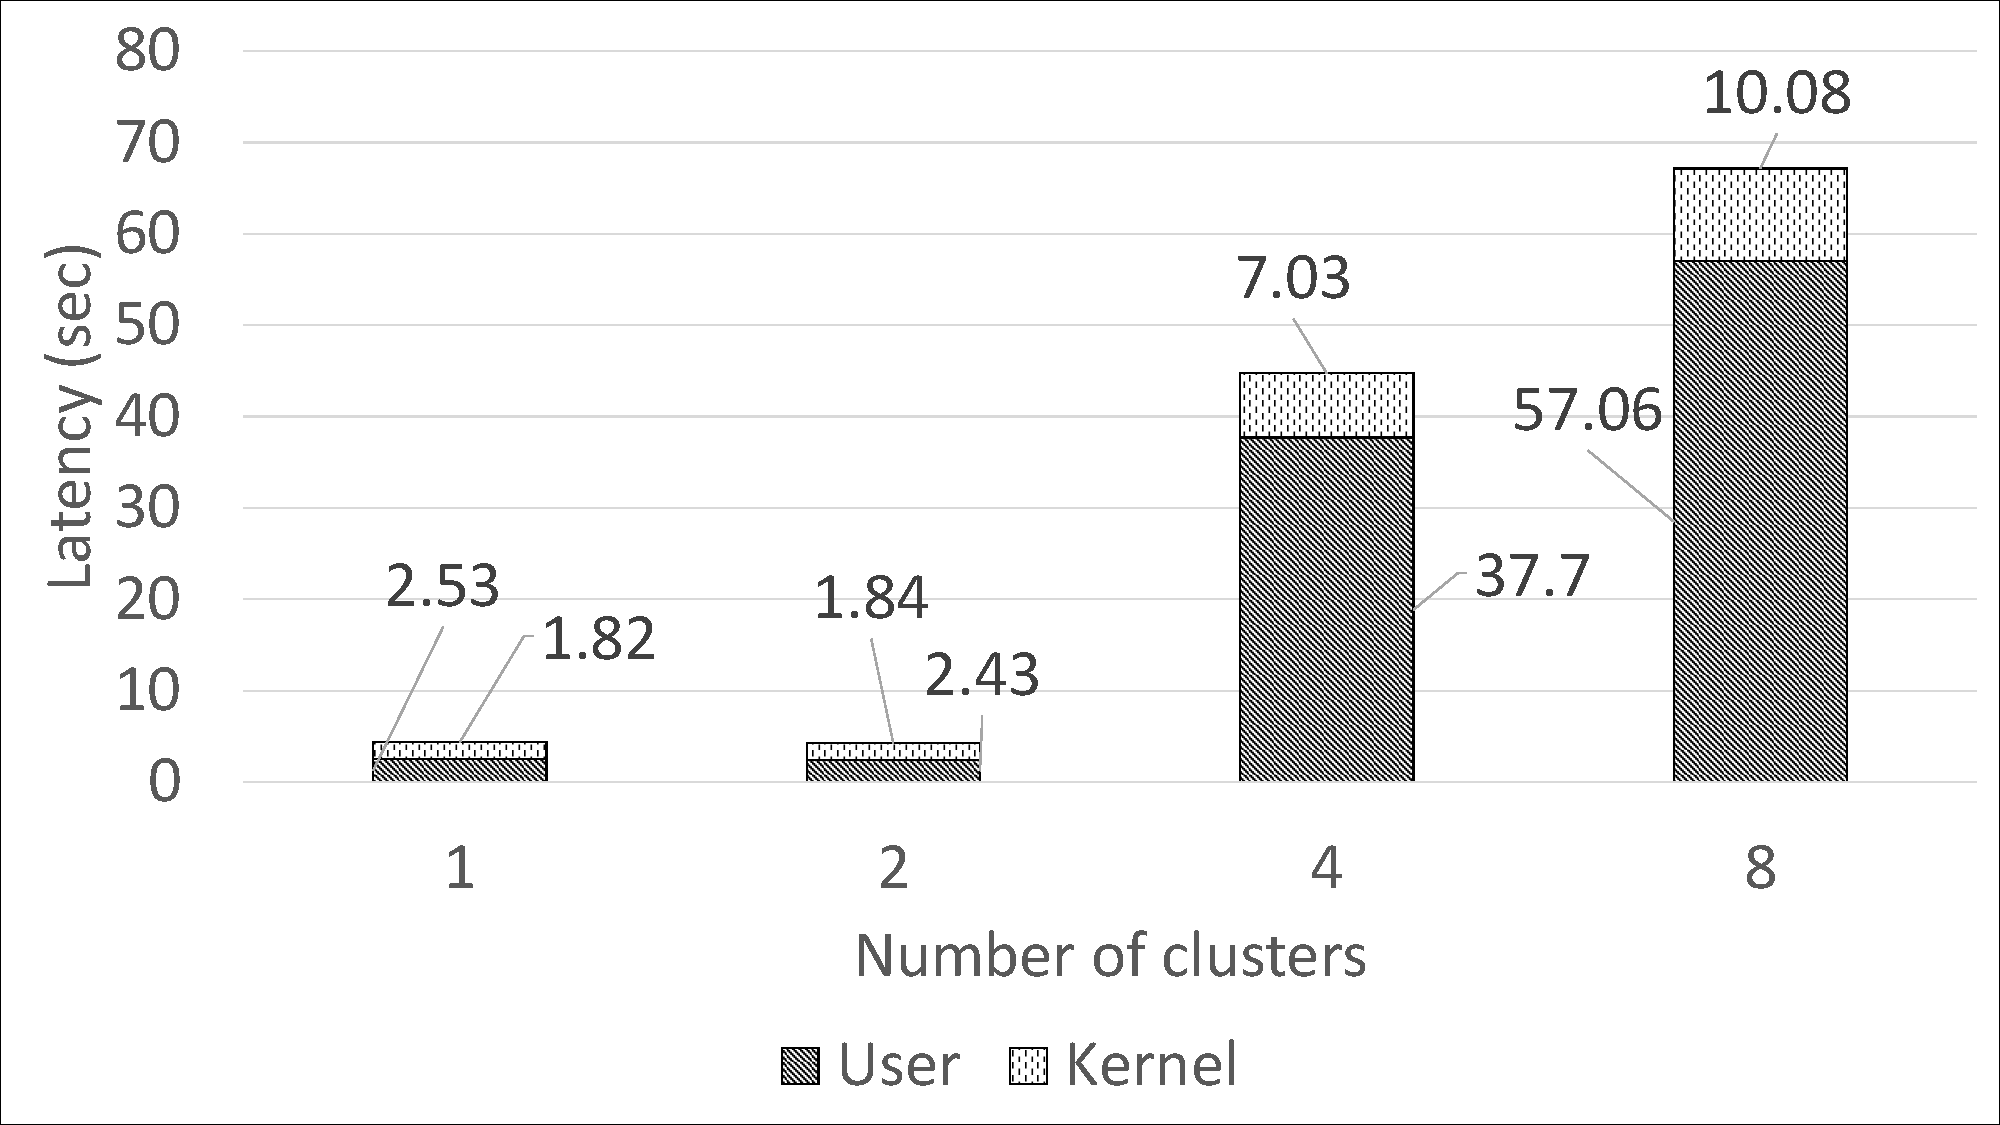
\includegraphics[width=0.4\textwidth]{evaluation/kmeans_latency_initial.pdf}}
       \subfigure[Latency (Agglomerative)\label{fig:agglomerative_init_latency}]
       {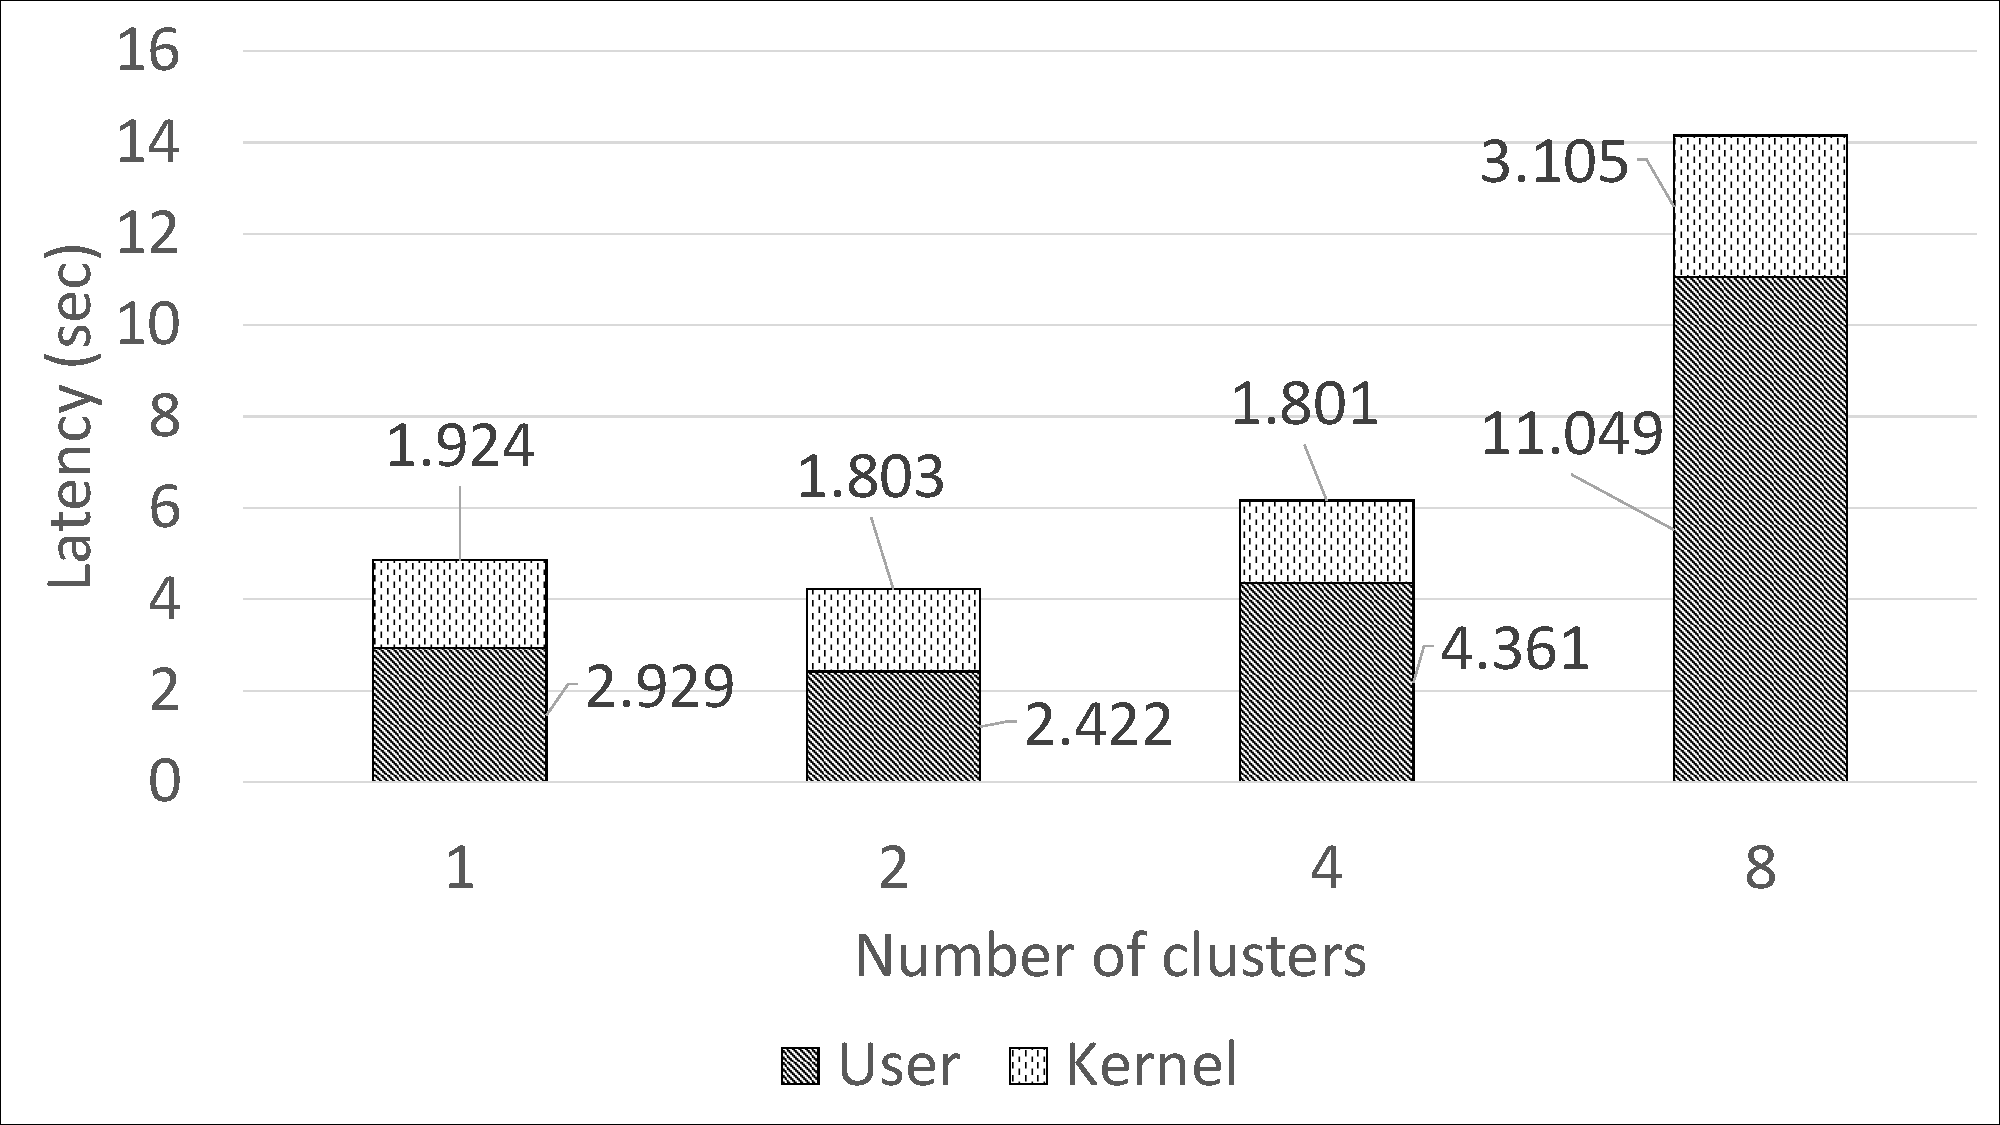
\includegraphics[width=0.4\textwidth]{evaluation/agglomerative_latency_initial.pdf}}
       \subfigure[Accuracy (K-means)\label{fig:kmeans_init_accuracy}]
       {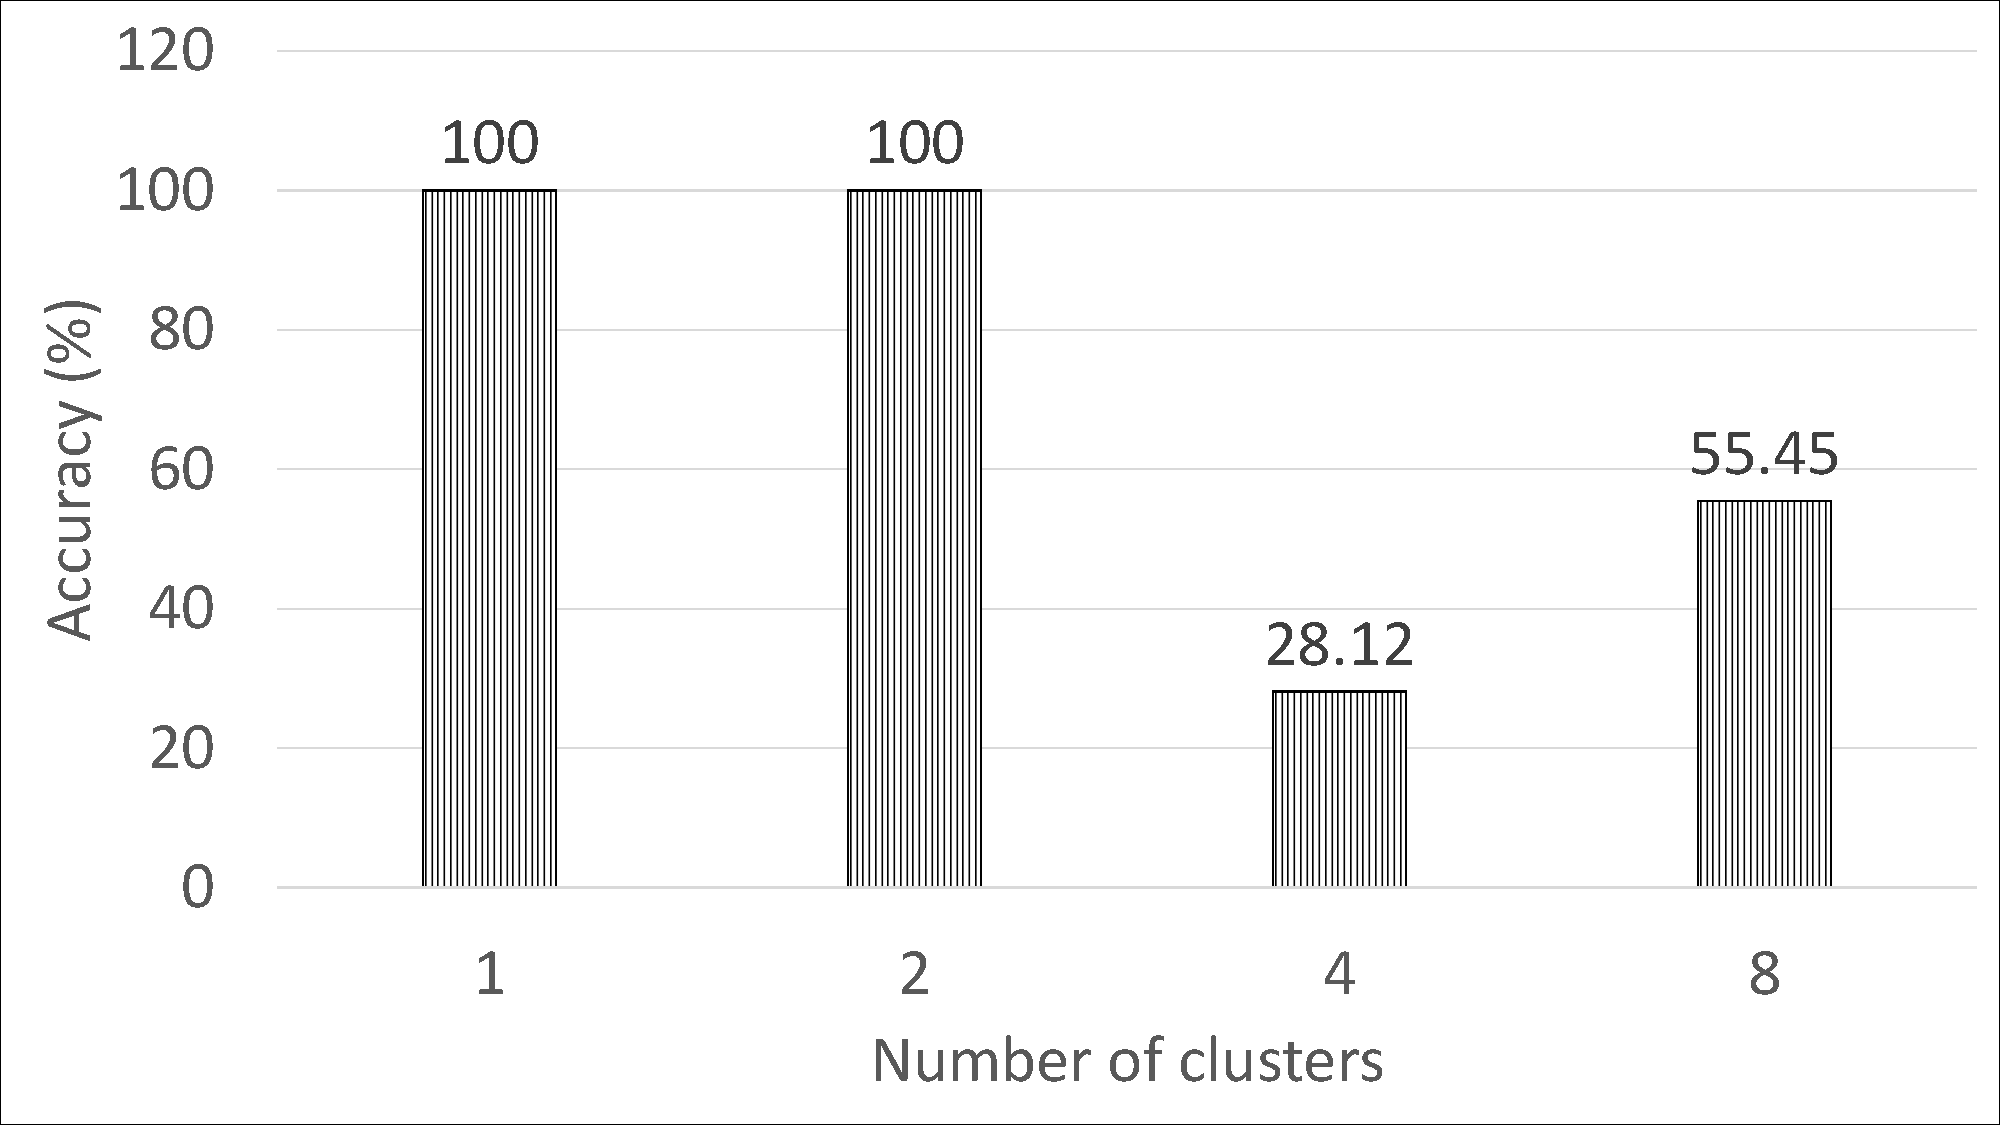
\includegraphics[width=0.4\textwidth]{evaluation/kmeans_accuracy_initial.pdf}}
       \subfigure[Accuracy (Agglomerative)\label{fig:agglomerative_init_accuracy}]
       {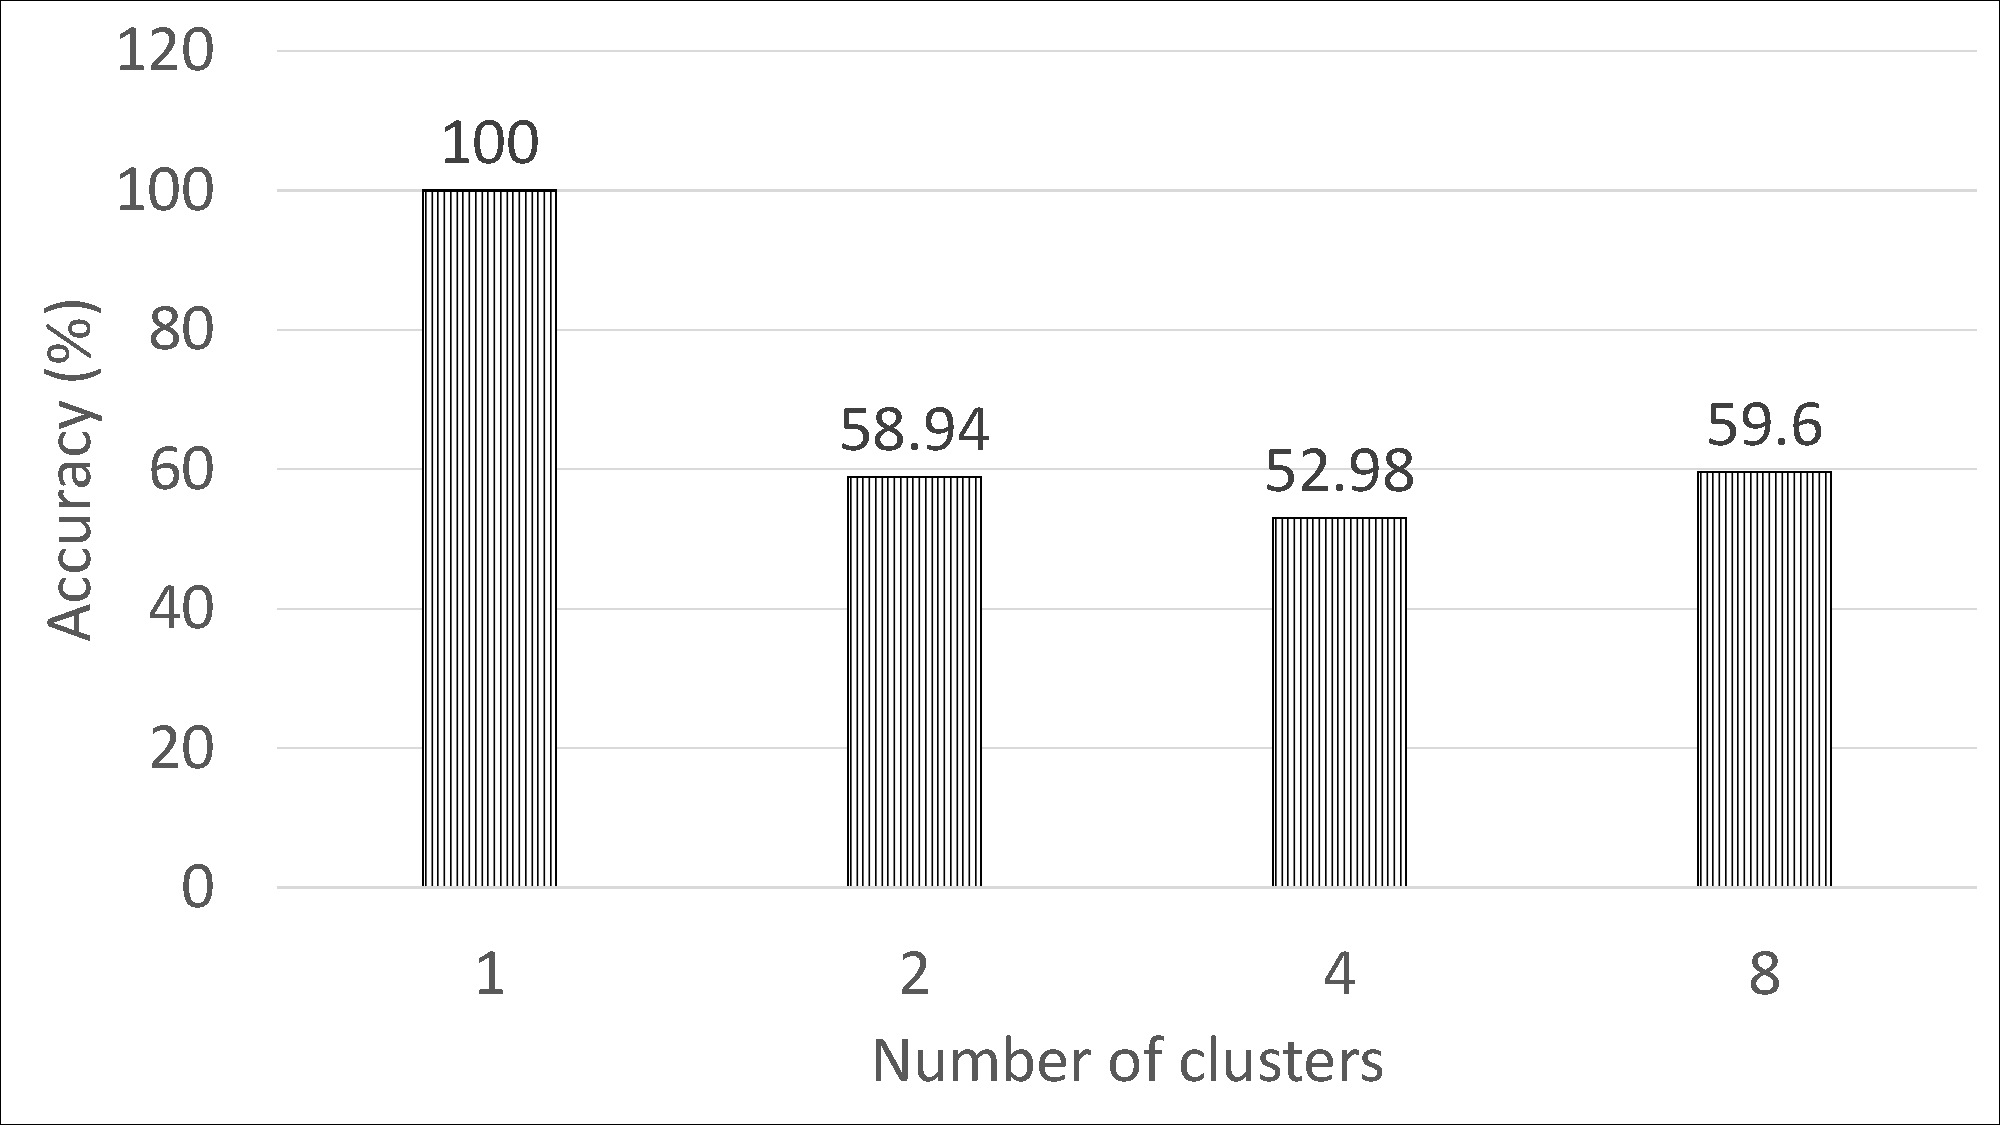
\includegraphics[width=0.4\textwidth]{evaluation/agglomerative_accuracy_initial.pdf}}
       \vspace{-0.0pc}
       \caption{Initial latency breakdown and accuracy for distributed shortest path detection algorithm on data clustered using K-means and Agglomerative clustering}
       \label{fig:init_eval}
    \end{center}
  \vspace{-1.0pc}
\end{figure*}

\begin{figure*}[h!]
    \vspace{-0.0pc}
    \begin{center}
        \subfigure[Latency (K-means)\label{fig:kmeans_impr_latency}]
        {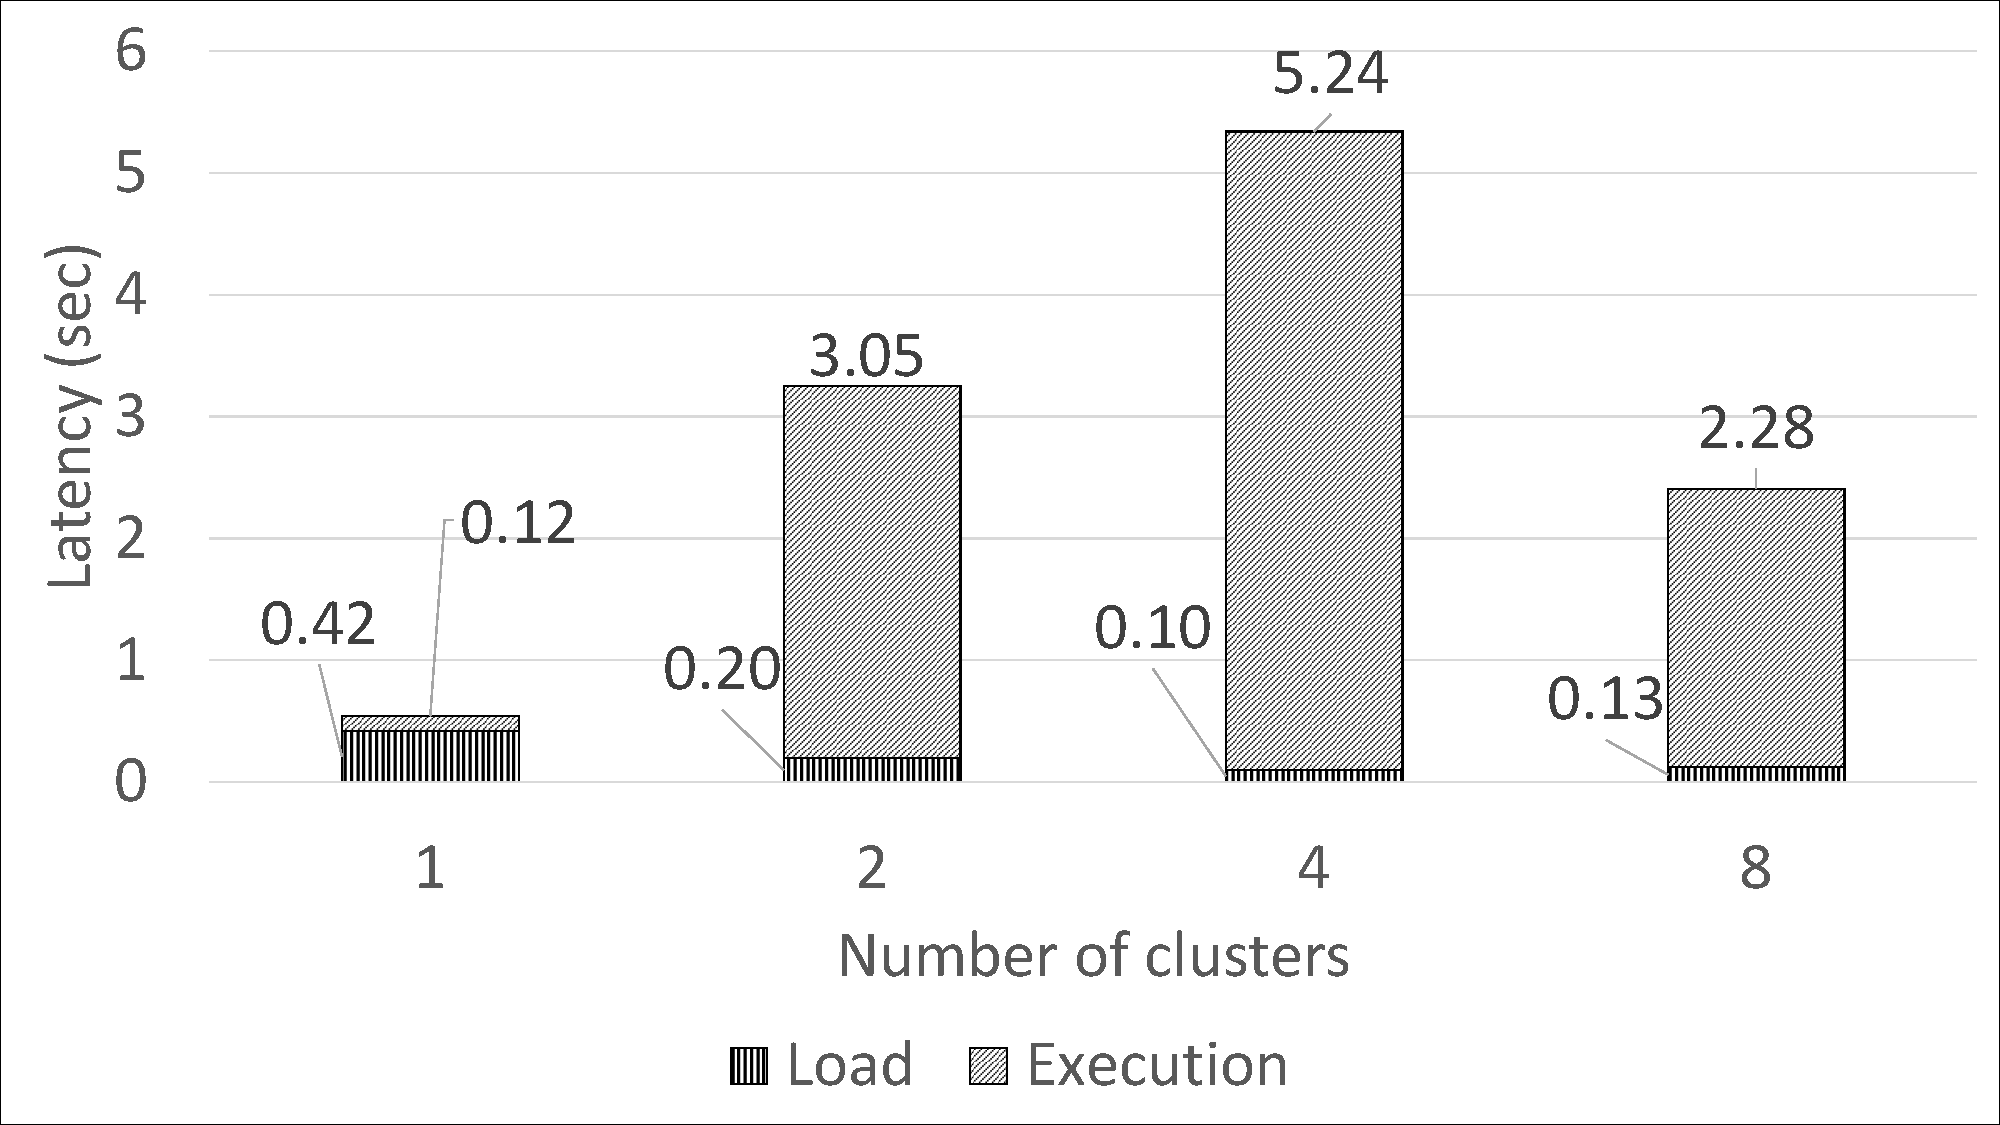
\includegraphics[width=0.4\textwidth]{evaluation/kmeans_latency.pdf}}
       \subfigure[Latency (Agglomerative)\label{fig:agglomerative_impr_latency}]
       {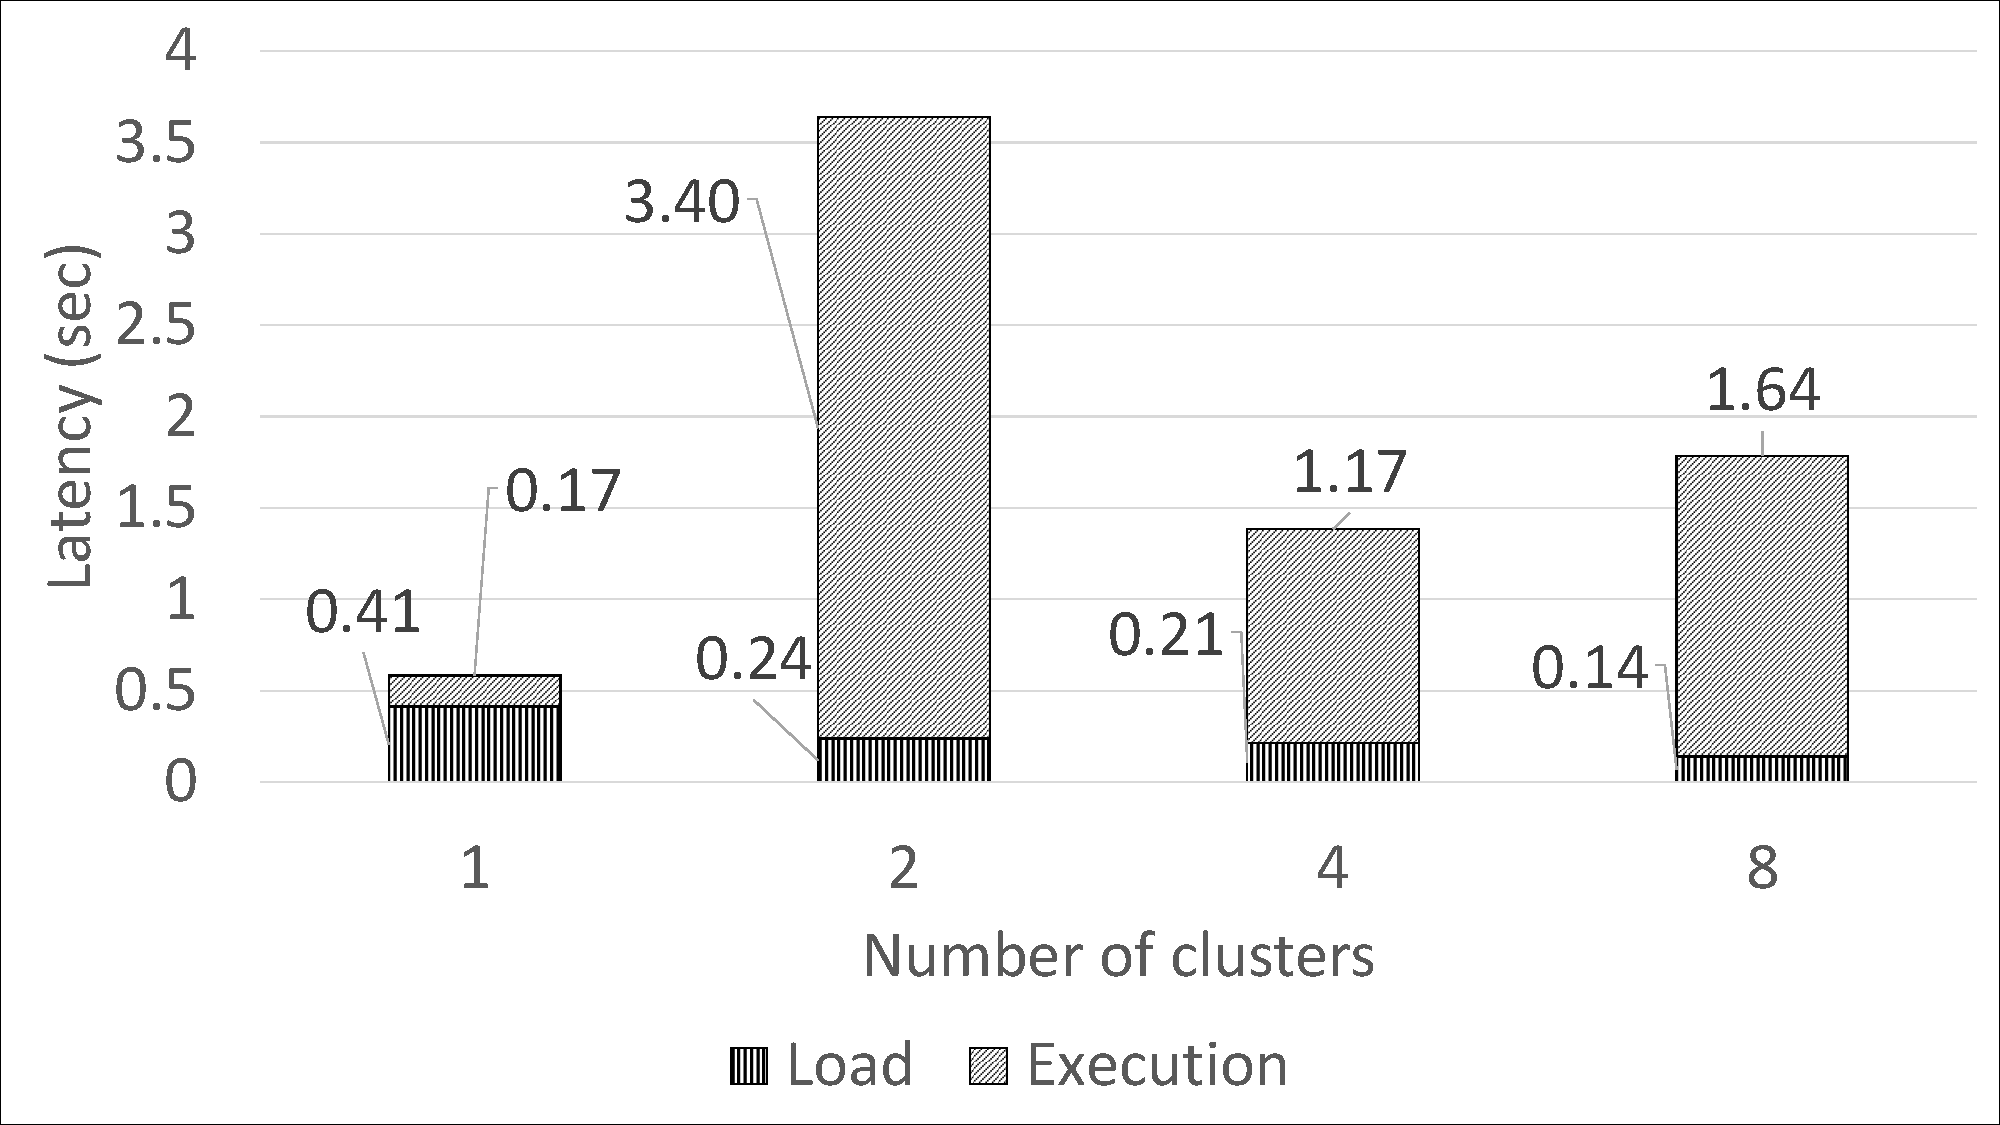
\includegraphics[width=0.4\textwidth]{evaluation/agglomerative_latency.pdf}}
       \subfigure[Accuracy (K-means)\label{fig:kmeans_impr_accuracy}]
       {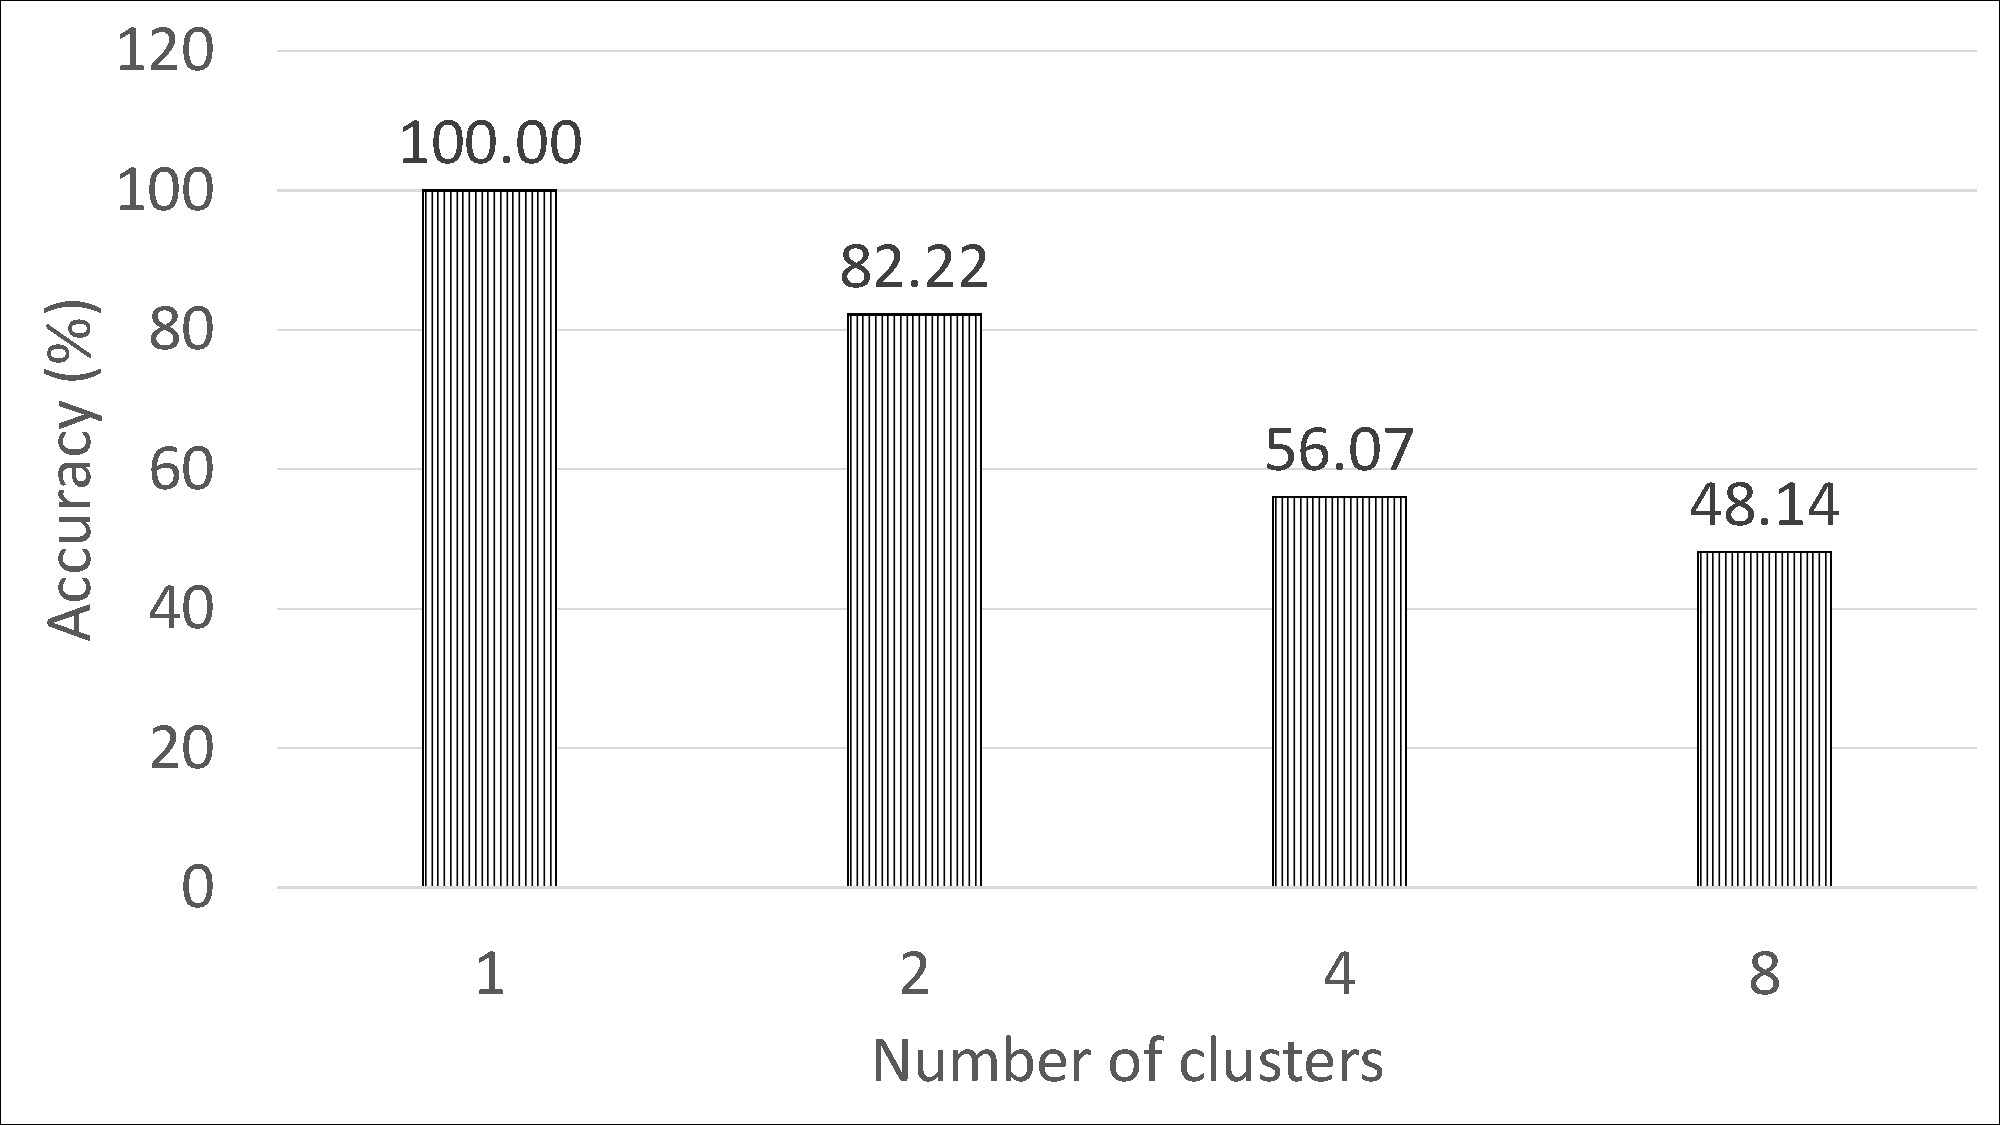
\includegraphics[width=0.4\textwidth]{evaluation/kmeans_accuracy.pdf}}
       \subfigure[Accuracy (Agglomerative)\label{fig:agglomerative_impr_accuracy}]
       {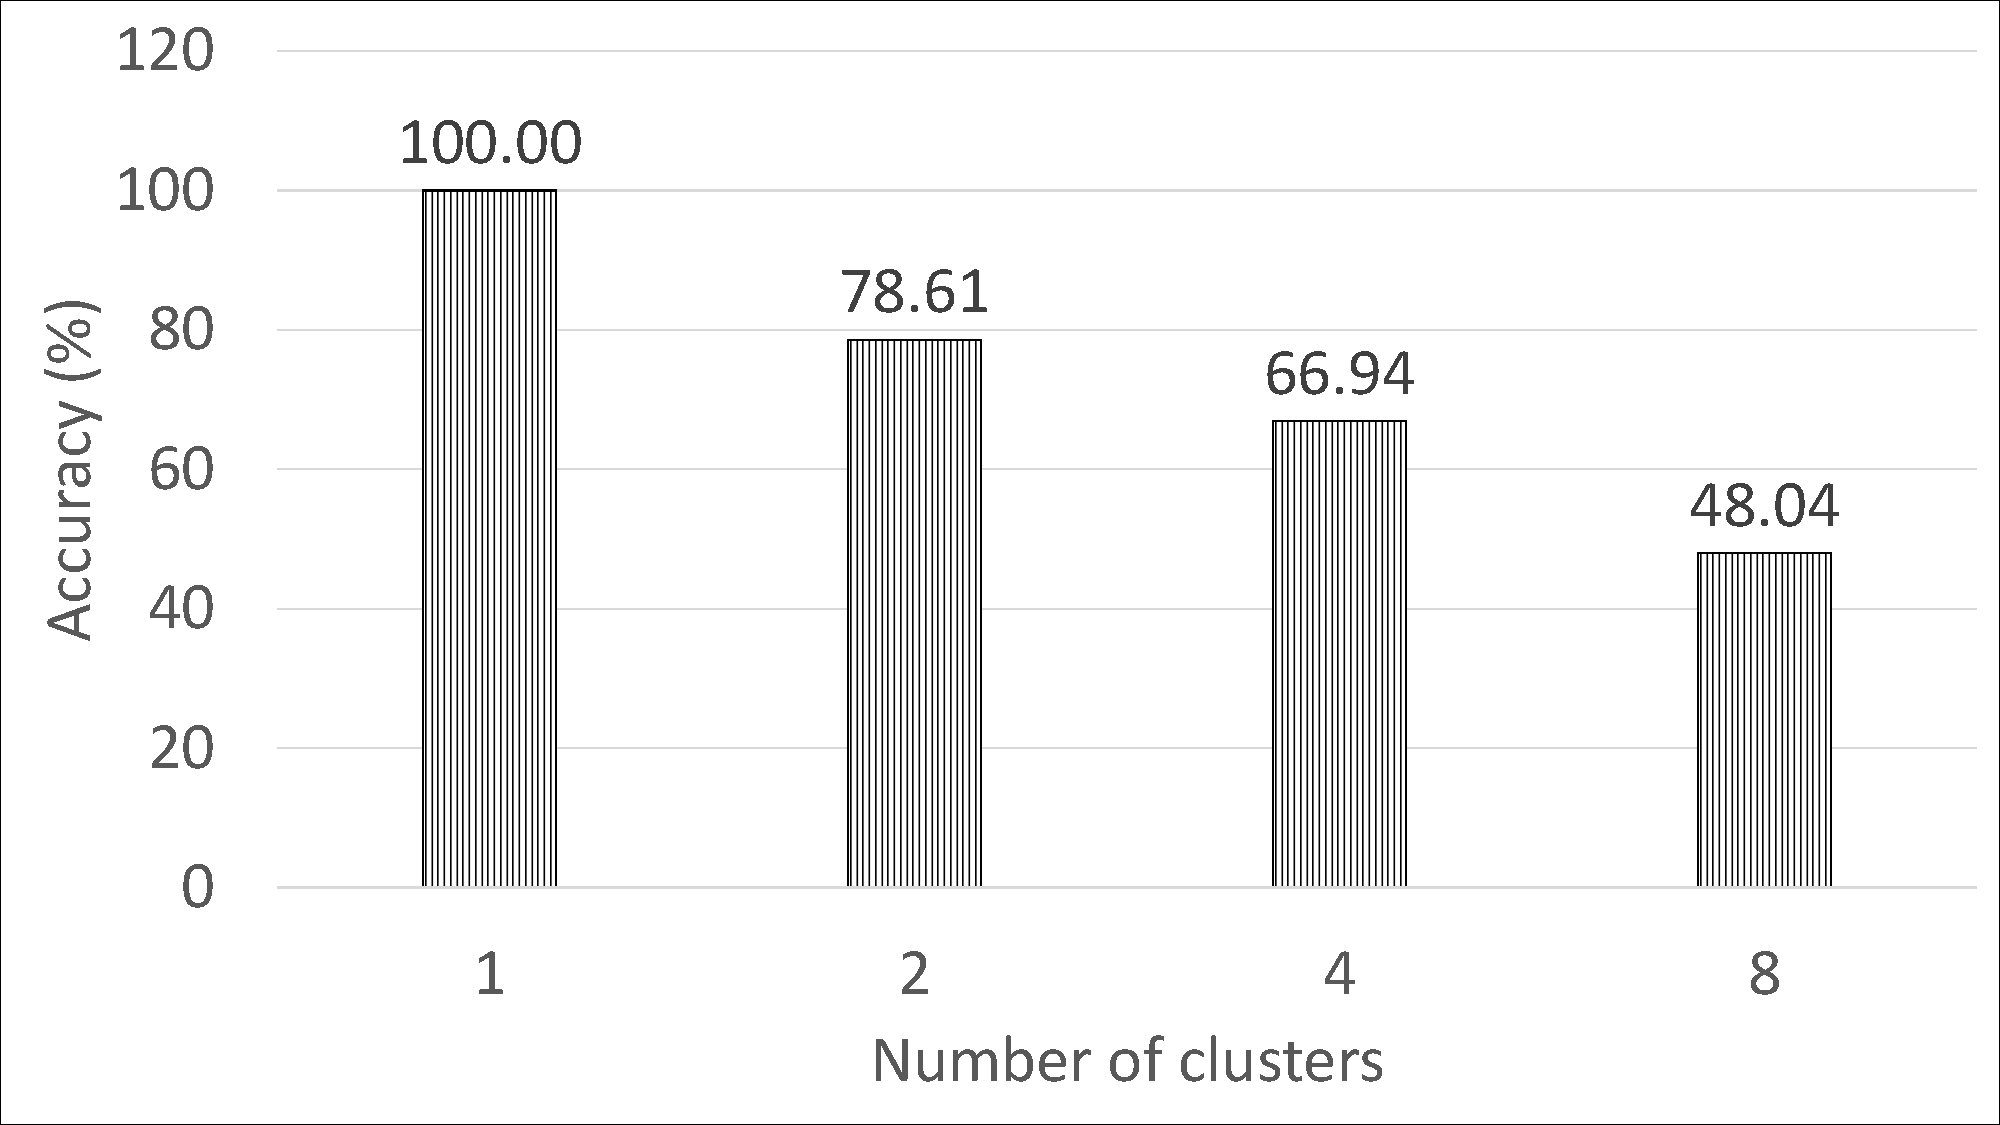
\includegraphics[width=0.4\textwidth]{evaluation/agglomerative_accuracy.pdf}}
       \vspace{-0.0pc}
       \caption{Improved latency breakdown and accuracy for distributed shortest path detection algorithm on data clustered using K-means and Agglomerative clustering}
       \label{fig:impr_eval}
    \end{center}
  \vspace{-1.0pc}
\end{figure*}

\subsubsection{Latency Evaluation}
\label{sec:latency_eval}
We measure the latency for both K-means and Agglomerative clustering in the initial implementation and the improved imeplementation.
In case of detecting the shortest path using the data clustered through K-means clustering, we observe that most of the latency
overhead occur in the user space. As shown in \figurename~\ref{fig:kmeans_init_latency} for K-means, with increasing number of clusters,
the time measured for the user space application execution increased drastically from 2.53 seconds for 1 cluster to 57.06 seconds
for 8 clusters, while the kernel space latency does not increase that much, i.e., from 1.82 seconds for 1 cluster to 10.08 seconds for 8 clusters.
Even though latency improvement was expected due to incorporating additional HPC resources, the high deependency among each
clusters for the geographic map data made difficult for the application and kernel to resolve the dependency among parallel units
of data. On the other hand, the data clustered using Agglomerative clustering technique behaved much better than that clustered using K-means.
For instance, as shown in \figurename~\ref{fig:agglomerative_init_accuracy}, the user space latency increased less steeply, i.e.,
from 2.93 seconds for 1 cluster to 11.049 seconds for 8 clusters. This is about 90\% improvement for 4 clusters and about 80\% improvement for
8 clusters. The kernel space latency also improved a lot for Agglomerative clustering. It was only 1.924 seconds for 1 cluster, stayed
almost the same for 2 and 4 clusters, and increased slightly to 3.1 seconds for 8 clusters.

Although we observed improvement by using data clustered by Agglomerative clustering technique, the latency measures were not only
higher than what we anticipated while planning the project, but also it was taking a lot of time in the user space. This means
there are problems in the algorithm implementation. After some profiling, we pinpointed the code snippet that was
creating performance bottleneck, i.e., the all source gateways to all destination gateways shortest path determination.
After this improvement, we ignored the kernel space latency and only focused on the user space latency. We further break the
latency down to data loading time from preprocessed pickle files and actual execution time of the distributed algorithm.
As shown in \figurename~\ref{fig:kmeans_impr_latency}, for K-means, the latency increased from 0.12 seconds for 1 cluster,
increased to 5.24 seconds for 4 clusters, and decreased to 2.28 seconds for 8 clusters. We observe about 56\% improvement
from cluster 4 to 8. On the other hand, for Agglomerative clustering, as stated in \figurename~\ref{fig:agglomerative_impr_latency},
the latency for the algorithm execution increased from 0.17 seconds for the whole graph to 3.40 seconds for 2 clusters.
Later, it had about 65\% decrement to 1.17 seconds for 4 clusters and increased a little to 1.64 seconds for 8 clusters.
For choosing Agglomerative clustering over K-means clustering, we can achieve about 78\% improvement in latency in this improved case.
For data loading time, it decreased slightly from 0.42 seconds for whole graph to 0.13 seconds for 8 clusters for K-means,
and 0.41 seconds for whole graph and 0.14 seconds for 8 clusters for Agglomerative clustering. This is obvious, because
with increased cluster numbers, we assign more HPC resources and each computing client have to read less amount of data.

\subsubsection{Accuracy Measurement}
\label{sec:accuracy_eval}
In the accuracy measurement, we compare the paths reported by the algorithm using the data from each clustering configuration
for different cluster numbers with the same path found from running the algorithm in 1 cluster or the whole graph.
We know that the whole graph contains all the connectivity and the path detected from whole graph is the ideal case scenario.
For calculating the output accuracy, we followed the equation below.
\[accuracy = n_c / n_i\]
where, $n_c$ = number of common nodes in ideal and given path, and $n_i$ = number of nodes in the ideal path.

As shown in \figurename~\ref{fig:kmeans_init_accuracy}, for K-means clustering, the accuracy is 100\% for 2 clusters,
but it drastically drops to 28.12\% for 4 clusters and got a little better to 55.45\% for 8 clusters.
On the contrary, for Agglomerative clustering, as depicted in \figurename~\ref{fig:agglomerative_init_accuracy},
we observed better accuracy trend than that for K-means clustered data, though it is quite less than what is expected
in general. For number of clusters more than 1, the accuracy stays in the range to 52.98\% to 59.6\%.

We measured the accuracy again after the code optimization discussed in Sec.~\ref{sec:latency_eval}.
This latency improvement impacted the accuracy a little, but in general it reported better accuracy
trend for different clustering configurations.
For instance, as shown in \figurename~\ref{fig:kmeans_impr_accuracy} for K-means clustering, the accuracy
dropped from 82.22\% to 48.14\% for 2 and 8 clusters respectively. For Agglomerative clustering, as depicted
in \figurename~\ref{fig:agglomerative_impr_accuracy}, it decreased from 78.61\% to 48.04\% for 2 and 8 clusters
respectively. Only for 4 clusters, data clustered by Agglomerative technique reports better accuracy (66.94\%) than
that (56.07\%) found by K-means data. In general, K-means and Agglomerative clustering demonstrate similar accuracy
trends.

\paragraph{Remarks}
The accuracy of the algorithm decreases with increasing number of clusters, because incorporating the clustered data
loses the inter-cluster connectivity information of the entire graph while running the algorithm in the
clustered data unit assigned to each process per client. Finally, after determining the final path by reducing
all the connectivity information via the gateway graph, we end up not finding the optimal solution. Nevertheless,
we get a suboptimal solution that represents a path from source node to the destination node.

\section{Conclusion and Future Work}
With the easy representability, graph has become a popular data structure for simplifying real world computation intensive problems. These real world problems are usually sequential and difficult to accelerate using modern distributed HPC systems. This work addresses graph parallelization problem, with the use of clustering approach by incorporating a master-slave architecture with the traditional single source shortest path algorithm. Our approach ensures data parallel execution of the algorithm in different partitions of the entire graph with a view to making it suitable for modern HPC systems. We have made a comparative analysis between partitioned-based and hierarchical clustering when applied on graph data structure. Our experiments show that hierarchical agglomerative clustering outperforms kmeans clustering in terms of accuracy and latency for graph parallelization. Due to the high connectivity among the different clusters of the graph data, the final reduction process to generate final output from the sub-outputs from each clusters is a challenging task even for the cutting edge HPC systems. There are still some scopes of improvement which we would like to leave as future work. Extending the existing clustering algorithms to reduce the inter-cluster edges can help us accelerate the proposed algorithm with better accuracy. Moreover, optimizing the gateway detection algorithm further can alleviate the latency degradation caused due to shortest path merging phase. Evaluating our approach for heuristic based algorithms, e.g., A* search, can also be an interesting line of study.
\label{sec:conclusion}
%\section{Expected Results}
\label{sec:expected_results}

In this project, the experiments will be run on the
in-house HPC system, \textit{Innovation}, at the Computer Architecture
and Systems Research Laboratory (CASTL). Multiple types of basic
shortest path algorithms will be implemented, and the runtime
performance and outcomes will be recorded.
Later, different clustering techniques will be applied to segregate
the dataset into subsets and algorithms described in Sec.~\ref{sec:methodology}
will be implemented. The parallel application will be run on \textit{Innovation}
such that each unit or component in the system deals with the data in each cluster.
Finally, all the separate results of each component will be aggregated and the total
runtime performance will be recorded. The final result for a specific
shortest path algorithm will be compared to the outcomes that were found
using the basic algorithm. Thus, the accuracy of the clustering technique will
be reported.

Hence, the research is expected to deliver the following results:
\begin{itemize}
    \item Application for clustering dataset, application to implement basic shortest path algorithms, parallel application to implement algorithm on clustered data.
    \item Runtime performance and outcomes from different basic shortest path algorith without clustering.
    \item Runtime performance and outcomes from different shortest path algorith with clustering.
    \item Intuitive comparison among differnt clustering techniques and the associated results.
    \item Evaluation of the accuracy of each clustering technique compared to the ideal results by the basic algorithms.
\end{itemize}

% \section{Possible Challenges}
\label{sec:challenges}

Dataset crisis

Clustering

Running on HPC

Accuracy
% \section{Timeline}
\label{sec:timeline}

The timeline of our project is depicted in Table~\ref{table:timeline}

\begin{table}[]
	\caption{Tentative Timeline}
	\begin{tabular}{|| c c ||} 
		\hline
		Task & Duration \\
		[0.5ex] 
		\hline\hline
        Literature Review & 1 week​ \\
        Dataset Analysis and Preprocessing​ & 1 week​ \\
		Implement Clustering​ & 2 weeks​ \\
		Implement Shortest Path Algorithms & 1 week​ \\
		Develop User Interface & 1 week​ \\
        Experimentation​ & 1 week​ \\
        Report Writing​ & 1 week​ \\[1ex] 
		\hline
	\end{tabular}
	\label{table:timeline}
\end{table}

\appendix

\subsection{OSM XML Data Format}
\label{app:osm_data}
\begin{verbatim}
	<?xml version="1.0"?>
	<osm version="0.6">
	<node id="298884269"
		lat="54.0901746"
		lon="12.2482632"
		uid="46882" ... />
		...
	</node> ...
	<way id="26659127" uid="55988" ...>
		<nd ref="292403538"/>
		<nd ref="298884289"/>
		...
		<tag k="highway"/>
	</way>
	</osm>
\end{verbatim}

\subsection{Data Structure}
\label{app:data_structure}
\begin{verbatim}
struct Cluster{​
int id;
list AdjacencyClusterList;
Cluster next_cluster;
float getClusterHeuristic(s,t);
};
struct Node{
int id;
float latitude;
float longitude;​
list AdjacencyList;
int cluster_id;
float getHeuristic(s,t)​;
};
\end{verbatim}
% needed in second column of first page if using \IEEEpubid
%\IEEEpubidadjcol

% An example of a floating figure using the graphicx package.
% Note that \label must occur AFTER (or within) \caption.
% For figures, \caption should occur after the \includegraphics.
% Note that IEEEtran v1.7 and later has special internal code that
% is designed to preserve the operation of \label within \caption
% even when the captionsoff option is in effect. However, because
% of issues like this, it may be the safest practice to put all your
% \label just after \caption rather than within \caption{}.
%
% Reminder: the "draftcls" or "draftclsnofoot", not "draft", class
% option should be used if it is desired that the figures are to be
% displayed while in draft mode.
%
%\begin{figure}[!t]
%\centering
%\includegraphics[width=2.5in]{myfigure}
% where an .eps filename suffix will be assumed under latex, 
% and a .pdf suffix will be assumed for pdflatex; or what has been declared
% via \DeclareGraphicsExtensions.
%\caption{Simulation Results}
%\label{fig_sim}
%\end{figure}

% Note that IEEE typically puts floats only at the top, even when this
% results in a large percentage of a column being occupied by floats.


% An example of a double column floating figure using two subfigures.
% (The subfig.sty package must be loaded for this to work.)
% The subfigure \label commands are set within each subfloat command, the
% \label for the overall figure must come after \caption.
% \hfil must be used as a separator to get equal spacing.
% The subfigure.sty package works much the same way, except \subfigure is
% used instead of \subfloat.
%
%\begin{figure*}[!t]
%\centerline{\subfloat[Case I]\includegraphics[width=2.5in]{subfigcase1}%
%\label{fig_first_case}}
%\hfil
%\subfloat[Case II]{\includegraphics[width=2.5in]{subfigcase2}%
%\label{fig_second_case}}}
%\caption{Simulation results}
%\label{fig_sim}
%\end{figure*}
%
% Note that often IEEE papers with subfigures do not employ subfigure
% captions (using the optional argument to \subfloat), but instead will
% reference/describe all of them (a), (b), etc., within the main caption.


% An example of a floating table. Note that, for IEEE style tables, the 
% \caption command should come BEFORE the table. Table text will default to
% \footnotesize as IEEE normally uses this smaller font for tables.
% The \label must come after \caption as always.
%
%\begin{table}[!t]
%% increase table row spacing, adjust to taste
%\renewcommand{\arraystretch}{1.3}
% if using array.sty, it might be a good idea to tweak the value of
% \extrarowheight as needed to properly center the text within the cells
%\caption{An Example of a Table}
%\label{table_example}
%\centering
%% Some packages, such as MDW tools, offer better commands for making tables
%% than the plain LaTeX2e tabular which is used here.
%\begin{tabular}{|c||c|}
%\hline
%One & Two\\
%\hline
%Three & Four\\
%\hline
%\end{tabular}
%\end{table}


% Note that IEEE does not put floats in the very first column - or typically
% anywhere on the first page for that matter. Also, in-text middle ("here")
% positioning is not used. Most IEEE journals use top floats exclusively.
% Note that, LaTeX2e, unlike IEEE journals, places footnotes above bottom
% floats. This can be corrected via the \fnbelowfloat command of the
% stfloats package.










% if have a single appendix:
%\appendix[Proof of the Zonklar Equations]
% or
%\appendix  % for no appendix heading
% do not use \section anymore after \appendix, only \section*
% is possibly needed

% use appendices with more than one appendix
% then use \section to start each appendix
% you must declare a \section before using any
% \subsection or using \label (\appendices by itself
% starts a section numbered zero.)
%


%\appendices
%\section{Proof of the First Zonklar Equation}
%\blindtext






% Can use something like this to put references on a page
% by themselves when using endfloat and the captionsoff option.
\ifCLASSOPTIONcaptionsoff
  \newpage
\fi



% trigger a \newpage just before the given reference
% number - used to balance the columns on the last page
% adjust value as needed - may need to be readjusted if
% the document is modified later
%\IEEEtriggeratref{8}
% The "triggered" command can be changed if desired:
%\IEEEtriggercmd{\enlargethispage{-5in}}

% references section

% can use a bibliography generated by BibTeX as a .bbl file
% BibTeX documentation can be easily obtained at:
% http://www.ctan.org/tex-archive/biblio/bibtex/contrib/doc/
% The IEEEtran BibTeX style support page is at:
% http://www.michaelshell.org/tex/ieeetran/bibtex/
%\bibliographystyle{IEEEtran}
% argument is your BibTeX string definitions and bibliography database(s)
%\bibliography{IEEEabrv,../bib/paper}
%
% <OR> manually copy in the resultant .bbl file
% set second argument of \begin to the number of references
% (used to reserve space for the reference number labels box)

\bibliographystyle{IEEEtran}
\bibliography{graph_dm_hpc}


% biography section
% 
% If you have an EPS/PDF photo (graphicx package needed) extra braces are
% needed around the contents of the optional argument to biography to prevent
% the LaTeX parser from getting confused when it sees the complicated
% \includegraphics command within an optional argument. (You could create
% your own custom macro containing the \includegraphics command to make things
% simpler here.)
%\begin{biography}[{\includegraphics[width=1in,height=1.25in,clip,keepaspectratio]{mshell}}]{Michael Shell}
% or if you just want to reserve a space for a photo:

%\begin{IEEEbiography}[{\includegraphics[width=1in,height=1.25in,clip,keepaspectratio]{picture}}]{John Doe}
%\blindtext
%\end{IEEEbiography}

% You can push biographies down or up by placing
% a \vfill before or after them. The appropriate
% use of \vfill depends on what kind of text is
% on the last page and whether or not the columns
% are being equalized.

%\vfill

% Can be used to pull up biographies so that the bottom of the last one
% is flush with the other column.
%\enlargethispage{-5in}




% that's all folks
\end{document}


